% !TEX encoding = UTF-8
% !TEX TS-program = pdflatex
% !TEX root = ../thesis.tex

%**************************************************************
\chapter{RISULTATI SPERIMENTALI}
\label{Capitolo4} \label{Chapter4}
\thispagestyle{empty}
Nel seguente capitolo vengono riportate le informazioni inerenti i vari datasets utilizzati in fase di addestramento. Oltre a questi, seguiranno tutti i risultati riguardanti le performance e i benefici prodotti dai modelli quando questi vengono sottoposti alle tecniche di compressione e non. Tutti i risultati ottenuti provengono dall'inferenza di vari modelli proiettati solo per il task di object detection.
Le specifiche delle architetture di riferimento utilizzate sono riportate nella Tabella (\ref{specifiche}).
\begin{table}
    \renewcommand{\baselinestretch}{1}
    \centering
    \begin{adjustbox}{max width=\textwidth}
    \begin{tabular}{|c||L|L|L||}
        \hline
        \multirow{2}{*}{\bfseries{ARCHITETTURE}} & \multicolumn{3}{c||}{\bfseries{SPECIFICHE TECNICHE}}\\            & \bfseries{CPU} & \bfseries{GPU} & \bfseries{RAM}\\
        \hline
        \hline
        {\bfseries{JETSON NANO}} & 4 $\times$ ARM Cortex-A57 @ 1.43 GHz & NVidia Maxwell @ 921 MHz & 4 GB 1600 MHz LPDDR4\\
        \hline
        {\bfseries{MACBOOK PRO}} & 8 $\times$ Intel Core i9 @ 2.3 GHz & AMD Radeon Pro 5500M @ 8 GB & 32 GB 2667 MHz DDR4\\
        \hline 
        {\bfseries{COLAB}} & 2 $\times$ Intel(R) Xeon(R) @ 2.20 GHz & NVidia Tesla P-100 @ 16 GB & 27 GB DDR4\\
        \hline
    \end{tabular}
    \end{adjustbox}
    \vspace{0.5cm}
    \caption{Specifiche tecniche delle tre architetture utilizzate.}
    \label{specifiche}
\end{table}
Al fine di mostrare i risultati raggiunti, il capitolo si conclude con una comparazione tra le performance dei modelli pre-addestrati e le performance del modello proposto, seguita da una carrellata di esempi prodotti da quest'ultimo.


\section{Descrizione dei dataset}\label{datasets_description}
Diversi sono i dataset utilizzati nell'ambito della guida autonoma.
Per quanto riguarda i modelli pre-addestrati, la loro formazione avviene con i seguenti datasets:
\begin{itemize}
    \item {\bfseries{\emph{CityScapes (CS)}}}\cite{Cityscapes}: i dati presenti in questo dataset sono composti da 
    diversi video stereo registrati nelle strade di 50 città diverse. Esistono 
    30 classi diverse raggruppate in otto categorie. Di queste immagini, 
    circa 5000 hanno annotazioni di alta qualità a livello di pixel, mentre altre 
    20.000 hanno annotazioni grossolane. Attualmente, questo dataset 
    rappresenta la pietra miliare della guida autonoma pertanto viene 
    utilizzato in molte ricerche. Nel presente elaborato, precisamente 
    nella sezione dei test di semantic segmentation, vengono utilizzate diverse 
    immagini appartenenti a codesto dataset (Fig. (\ref{cityscapes})), ognuna opportunamente ridimensionata ad una risoluzione diversa.
    \begin{figure}
        \centering
        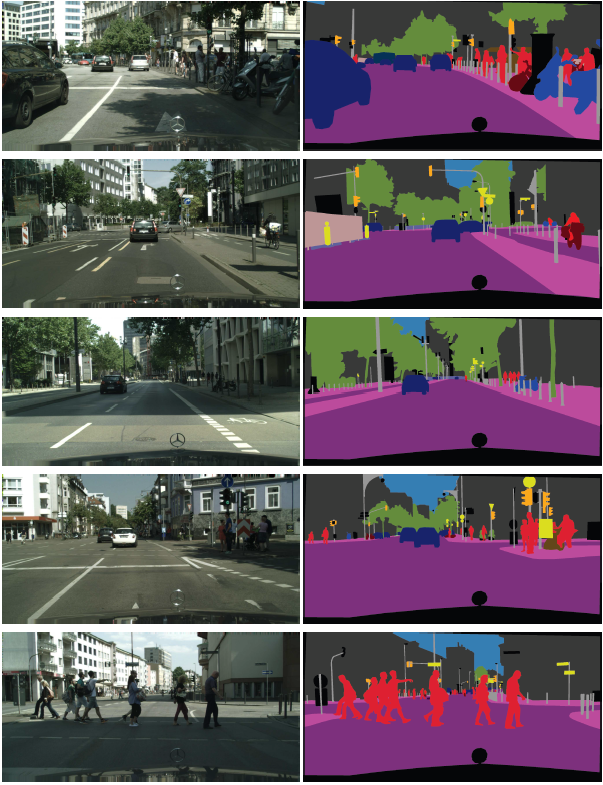
\includegraphics[width = \linewidth]{cityscapes4.png}
        \centering
        \caption{Esempio di immagini presenti in Cityscapes. A destra viene mostrata l'immagine originale mentre a sinistra la sua segmentazione semantica (Ground Truth).}
        \label{cityscapes}
    \end{figure} 
    ($512\times 256$, $1024\times 512$, $2048\times 1024$).
    \item {\bfseries{\emph{PASCAL Visual Object Classes (VOC)}}}\cite{VOC}: il seguente dataset 
    contiene più di 10.000 immagini con all'interno un totale di più di 20.000 
    oggetti raggruppati in 20 classi diverse (Fig. \ref{pascal}). Anche questo dataset, come 
    il precedente, viene utilizzato nella sezione di test per il task di 
    semantic segmentation in questo elaborato. Dettagliatamente, vengono 
    utilizzate delle sue immagini ridimensionate in formato $320\times 320$ e $512\times 320$.
    \begin{figure}
        \centering
        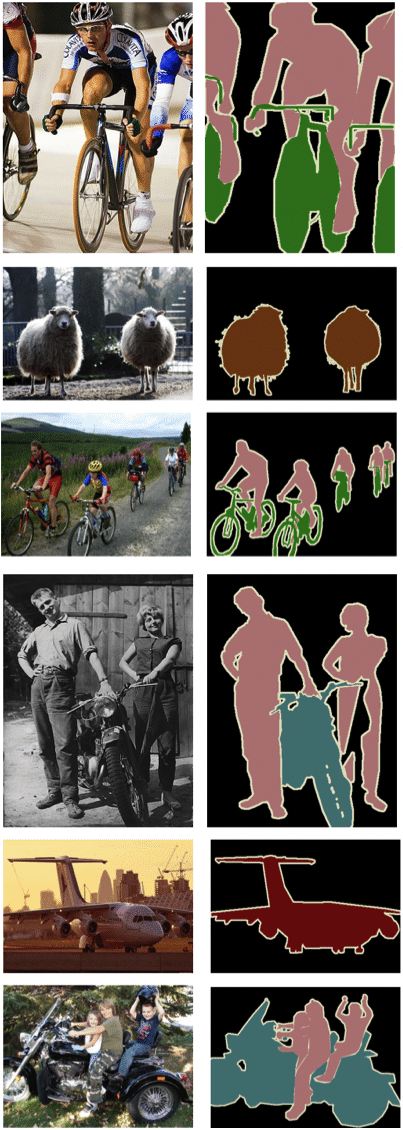
\includegraphics[width = 0.5\linewidth]{PascalVOC.png}
        \centering
        \caption{Esempio di immagini presenti in Pascal VOC. A destra viene mostrata l'immagine originale mentre a sinistra la sua segmentazione semantica (Ground Truth).}
        \label{pascal}
    \end{figure} 
    \item {\bfseries{\emph{MS Common Objects in Context (COCO)}}}\cite{COCO}: realizzato da 
    Microsoft, il dataset contiene più di 300.000 immagini di cui più di 
    200.000 sono etichettate (Fig. (\ref{MSCOCO_dataset})). Gli oggetti presenti sono più di 1.5 milioni e 
    sono raggruppati in 150 classi diverse. Principalmente questo dataset 
    viene utilizzato per attività di object detection, infatti ritorna utile 
    nella sezione di test successiva. La risoluzione standard delle immagini presenti è pari a 640x480.
    \begin{figure}
        \centering
        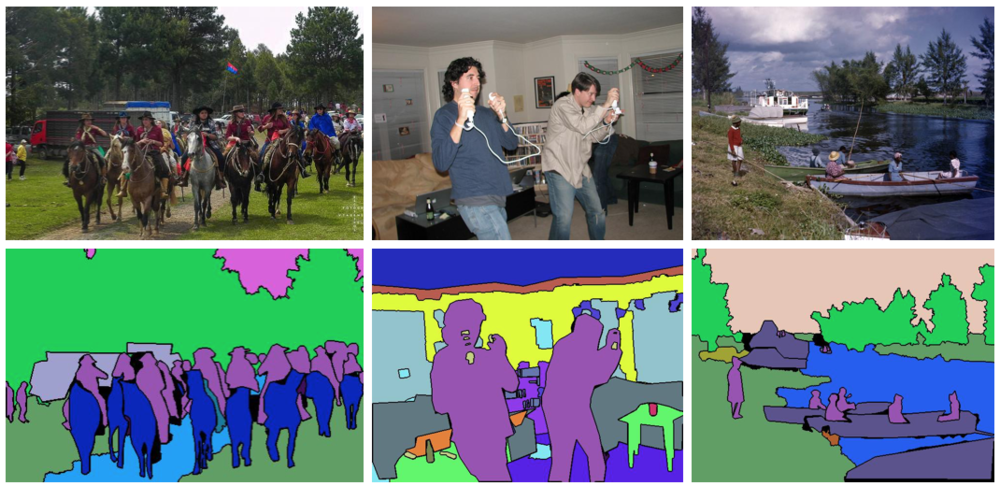
\includegraphics[width = \linewidth]{MSCOCO.png}
        \centering
        \caption{Esempio di immagini presenti in MS COCO. A destra viene mostrata l'immagine originale mentre a sinistra la sua segmentazione semantica (Ground Truth).}
        \label{MSCOCO_dataset}
    \end{figure} 
    Sia l'allenamento del modello base che dell'intero modello proposto, avviene tramite l'utilizzo del seguente dataset:
    \item {\bfseries{\emph{Open Images}}}\cite{OpenImages2}: dataset utilizzato per lo più in ambito di object detection e semantic segmentation (Fig. \ref{openimages_dataset}). La rete base integrata nel modello proposto, pur essere concepita per svolgere attività di image classification, ha utilizzato ugualmente le immagini di codesto dataset. Per il modello di riferimento invece, lo script utilizzato per il reperimento delle immagini ha fornito anche le informazioni di ogni bounding-box raffigurante il riquadro di delimitazione di ogni oggetto in ogni immagine. Attualmente, il dataset fornisce oltre 6000 categorie per un totale di 9 milioni di immagini etichettate. La risoluzione delle immagini è molto variabile ma, rispetto agli altri datasets, è possibile trovare immagini ad un'alta risoluzione come 3000x2267.
    Per quanto concerne l'attività di object detection, il dataset è in grado di fornire 16 milioni di bounding-boxes inerenti 600 categorie di oggetti su un totale di 1.9 milioni di immagini. Questi dati lo piazzano in prima posizione come dataset più numeroso. 
    \begin{figure}
        \centering
        \includegraphics[width = 0.6\linewidth]{open_images_figure.png}
        \centering
        \caption{Esempio di immagine presente in Open Images. Sull'immagine vengono sovolte contemporaneamente le attività di object detection e di semantic segmentation.}
        \label{openimages_dataset}
    \end{figure}
\end{itemize}

\section{Accuratezza tecniche di compressione/ottimizzazione}
In questa nuova sezione verranno analizzati i livelli di accuratezza raggiunti da entrambe le tecniche di compressione utilizzate. Lo studio vuole mettere in risalto i benefici introdotti da tali tecniche su tutti quei dispositivi limitati a livello di risorse hardware.
Successivamente verranno mostrati i risultati ottenuti prima sulla tecnica di Pruning e successivamente sulla tecnica di Knowledge Distillation\index{Knowledge Distillation}.

\subsection{Accuratezza Pruning}
Più che accuratezza, la tecnica di pruning è utile a mostrare i risultati inerenti la funzione di perdita di un modello, che a loro volta sono strettamente correlati all'accuratezza raggiunta. Quando l'accuratezza di un modello incomincia a degradarsi, allo stesso modo peggiorerà la sua funzione di perdita. Il modello su cui è stata applicata la seguente tecnica è l'\emph{SSD-MobileNet-V1} (Sez. \ref{MBNET}).
Si ricorda che tale modello è stato costruito da zero ("from scratch") ed è stato addestrato, su un totale di 1000 epoche, utilizzando le immagini del dataset Open Images.
Come già accennato nei capitoli precedenti, l'applicazione di tale tecnica può avvenire secondo tre metodi diversi: \emph{Structured}, \emph{Unstructured} e \emph{Global Unstructured}.
Essendo un modello congruo per l'attività di object detection, per ogni metodo vengono calcolate tre tipologie di perdite: \emph{Globale}, di \emph{Classificazione} e di \emph{Regressione}.
Partendo dal metodo \emph{Structured}, che ricordo agire solamente sui filtri, nonché i canali convoluzionali, tutte le perdite del modello incominciano ad aumentare quando si arriva ad utilizzare un indice di sparsità compreso tra il 10-15\% (Fig. \ref{struct_loss_global_pruning}, Fig. \ref{struct_loss_class_pruning}, Fig.\ref{struct_loss_regr_pruning}). I riferimenti dettati nella sezione \ref{pruning_model}, appaiono quindi essere confermati dai valori riportati nei grafici i quali, a loro volta, schedulano tale metodologia di pruning come inaccurata per ricavare informazioni. 
Cambiando metodologia, ci si concentra ora sulla tecnica \emph{Unstructured}. La seguente mira direttamente ad azzerare specifici parametri, come pesi e bias, presenti nella rete. I risultati ottenuti indicano uno scenario del tutto diverso rispetto a quello risultante dalla tecnica precedente. Questa volta, prima che l'accuratezza diverga, l'indice di sparsità aumenta, portandosi a raggiungere un valore del 40\% (Fig. \ref{unstr_loss_global_pruning}, Fig. \ref{unstr_loss_class_pruning} Fig. \ref{unstr_loss_regr_pruning}). Questo sta a significare un netto aumento del numero di parametri che possono essere azzerati e di conseguenza eliminati. 
Gli ultimi risultati mostrati, riguardano quelli derivanti dalla tecnica \emph{Global Unstructured}. La tecnica si concentra nell'applicare un'intera quantità di sparsità, un'unica volta, in tutto il modello. Considerata tra le più affidabili rispetto alle due precedenti, la tecnica rappresenta un vero e proprio set di parametri che possono essere rimossi dal modello. Dai risultati mostrati, capiamo come molti dei pesi presenti sono in realtà superflui. Prima che l'accuratezza degradasse, la rimozione del 60\% (Fig. \ref{glob_loss_global_pruning}, Fig. \ref{glob_loss_class_pruning}, Fig. \ref{glob_loss_regr_pruning}) dei pesi presenti porterebbe ad un balzo significativo delle performance del modello.
Tirando le somme, data la significativa grandezza del modello, una tale riduzione, pari a più della metà dei parametri, dimostra come ci sia ancora tanta strada da percorrere per arrivare all'ottenimento un modello ottimale. Secondo il parere del sottoscritto, molto probabilmente, i risultati ottenuti non cambierebbero se la rete SSD avesse avuto una rete base diversa da MobileNet-V1.
\begin{figure}
    \centering
    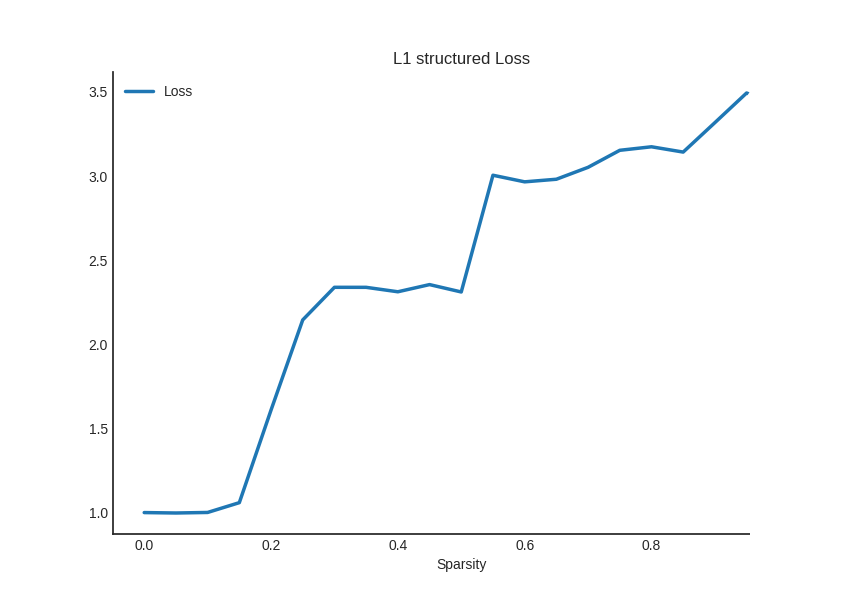
\includegraphics[width = \linewidth]{structured_Loss.png}
    \centering
    \caption{Perdita globale Structuerd Pruning.}
    \label{struct_loss_global_pruning}
\end{figure}
\begin{figure}
    \centering
    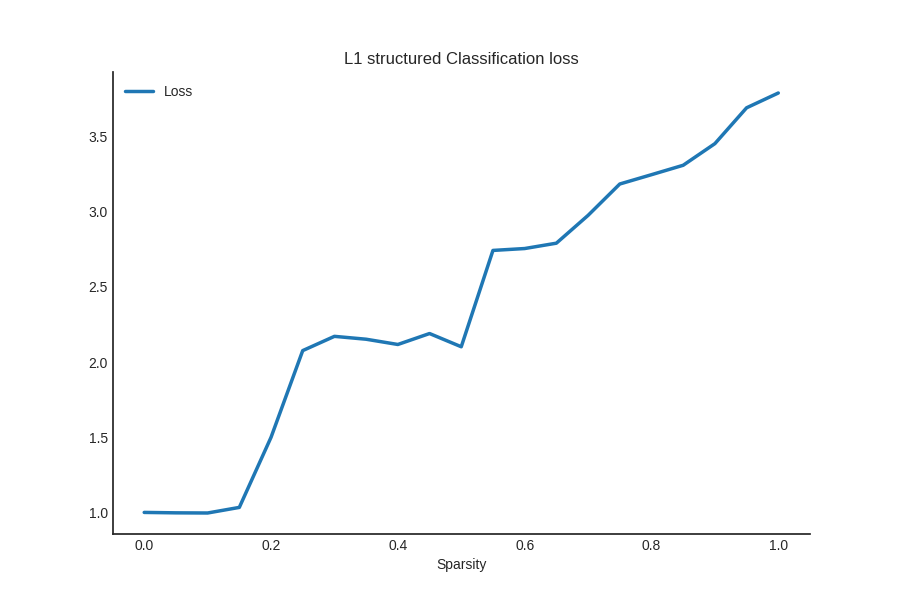
\includegraphics[width = \linewidth]{structured_ClassLoss.png}
    \centering
    \caption{Perdita classificazione Structuerd Pruning.}
    \label{struct_loss_class_pruning}
\end{figure}
\begin{figure}
    \centering
    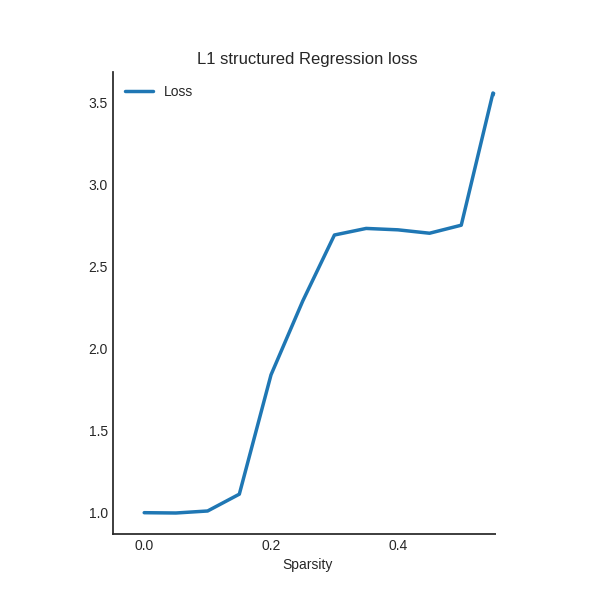
\includegraphics[width = 0.7\linewidth]{structured_RegrLoss.png}
    \centering
    \caption{Perdita regressione Structuerd Pruning.}
    \label{struct_loss_regr_pruning}
\end{figure}
\begin{figure}
    \centering
    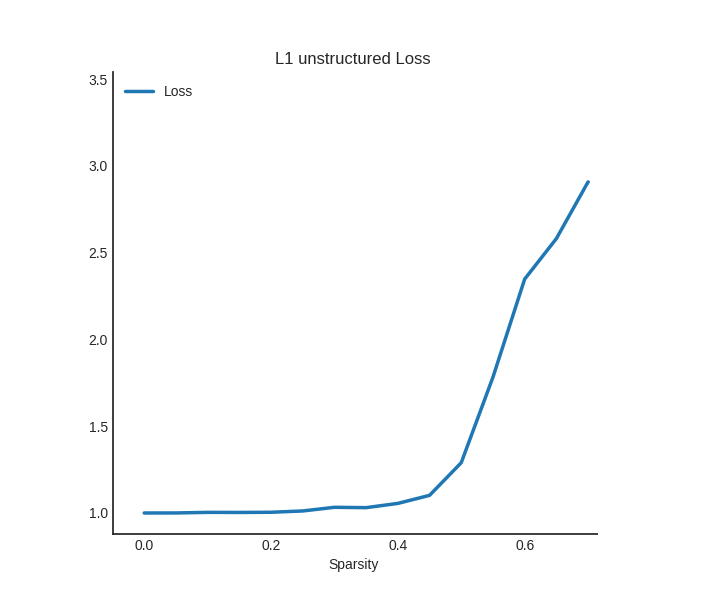
\includegraphics[width = 0.8\linewidth]{unstructured_Loss.png}
    \centering
    \caption{Perdita globale Unstructuerd Pruning.}
    \label{unstr_loss_global_pruning}
\end{figure}
\begin{figure}
    \centering
    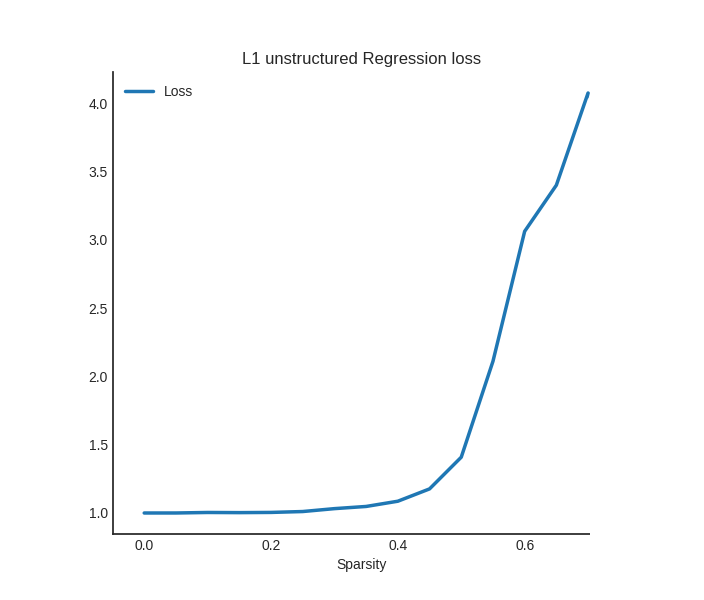
\includegraphics[width = 0.8\linewidth]{unstructured_ClassLoss.png}
    \centering
    \caption{Perdita classificazione Unstructuerd Pruning.}
    \label{unstr_loss_class_pruning}
\end{figure}
\begin{figure}
    \centering
    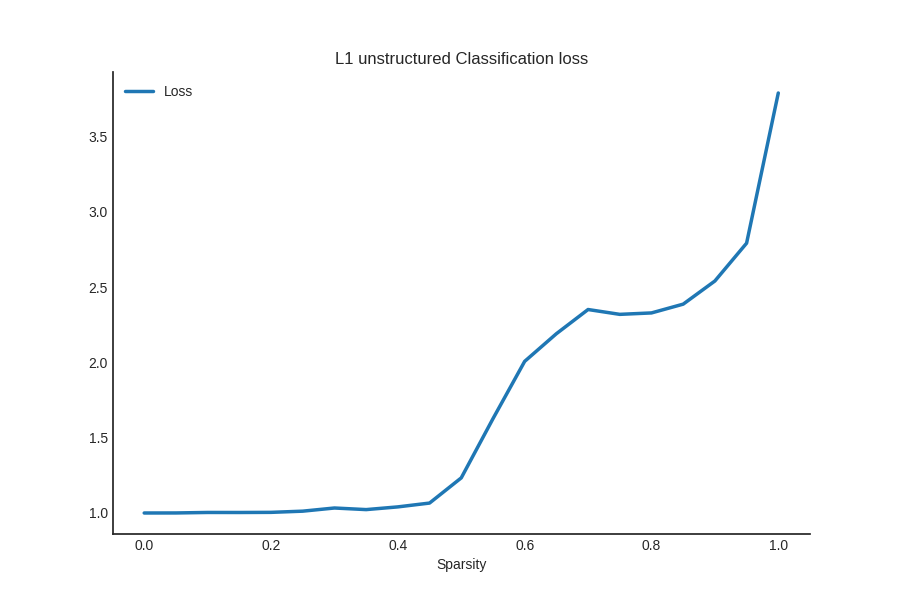
\includegraphics[width = \linewidth]{unstructured_RegrLoss.png}
    \centering
    \caption{Perdita regressione Unstructuerd Pruning.}
    \label{unstr_loss_regr_pruning}
\end{figure}
\begin{figure}
    \centering
    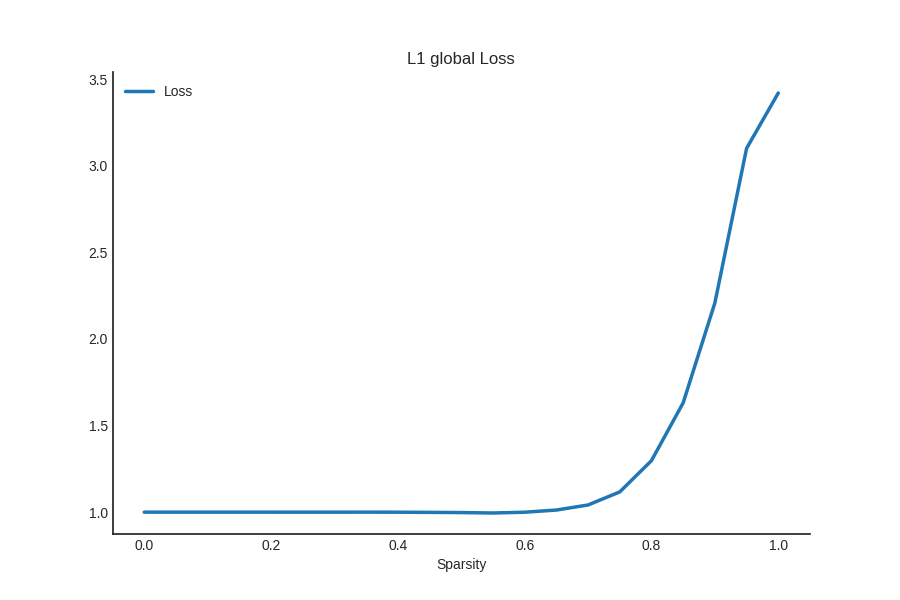
\includegraphics[width = \linewidth]{global_Loss.png}
    \centering
    \caption{Perdita complessiva Global Unstructuerd Pruning.}
    \label{glob_loss_global_pruning}
\end{figure}
\begin{figure}
    \centering
    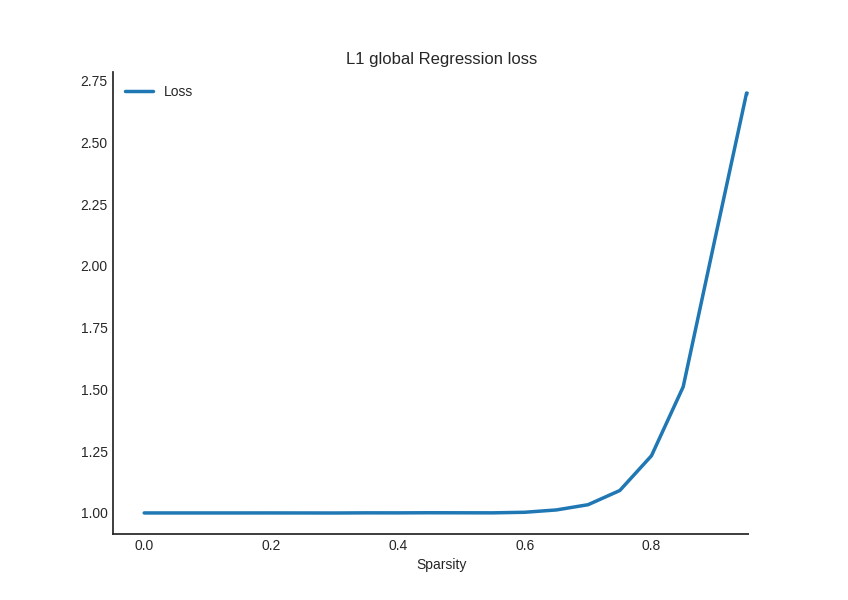
\includegraphics[width = \linewidth]{global_ClassLoss.png}
    \centering
    \caption{Perdita classificazione Global Unstructuerd Pruning.}
    \label{glob_loss_class_pruning}
\end{figure}
\begin{figure}
    \centering
    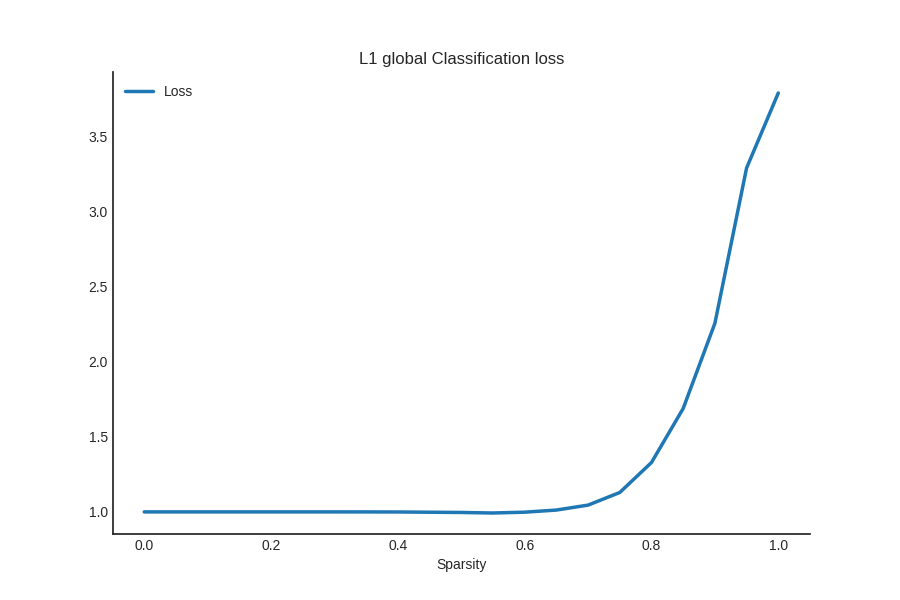
\includegraphics[width = \linewidth]{global_RegrLoss.png}
    \centering
    \caption{Perdita regressione Global Unstructuerd Pruning.}
    \label{glob_loss_regr_pruning}
\end{figure}

\subsection{Accuratezza Knowledge Distillation}\index{Knowledge Distillation}
La seconda tecnica di compressione/ottimizzazione, nonché la più approfondita a livello pratico, si è dimostrata da subito una sfida ardua da affrontare. Stando al procedimento descritto nella sezione \ref{KD_steps}, l'obiettivo è quello di trovare il miglior modello studente distillato tra quelli generati ad una temperatura variabile. L'unico modo per ricercare tale modello è mediante la comparazione dell'accuratezza di ognuno di loro. Ricordo che il vincolo imposto obbligava a scegliere un modello la cui temperatura di generazione fosse maggiore di uno. Le accuratezze vengono calcolate corrispettivamente sulle predizioni Top-1 e Top-5 restituite e riportate sia sottoforma di grafico (Fig. \ref{accuracy_KD} che tabellare (Tab. \ref{accuracy_models_dist}).
\begin{figure}
    \centering
    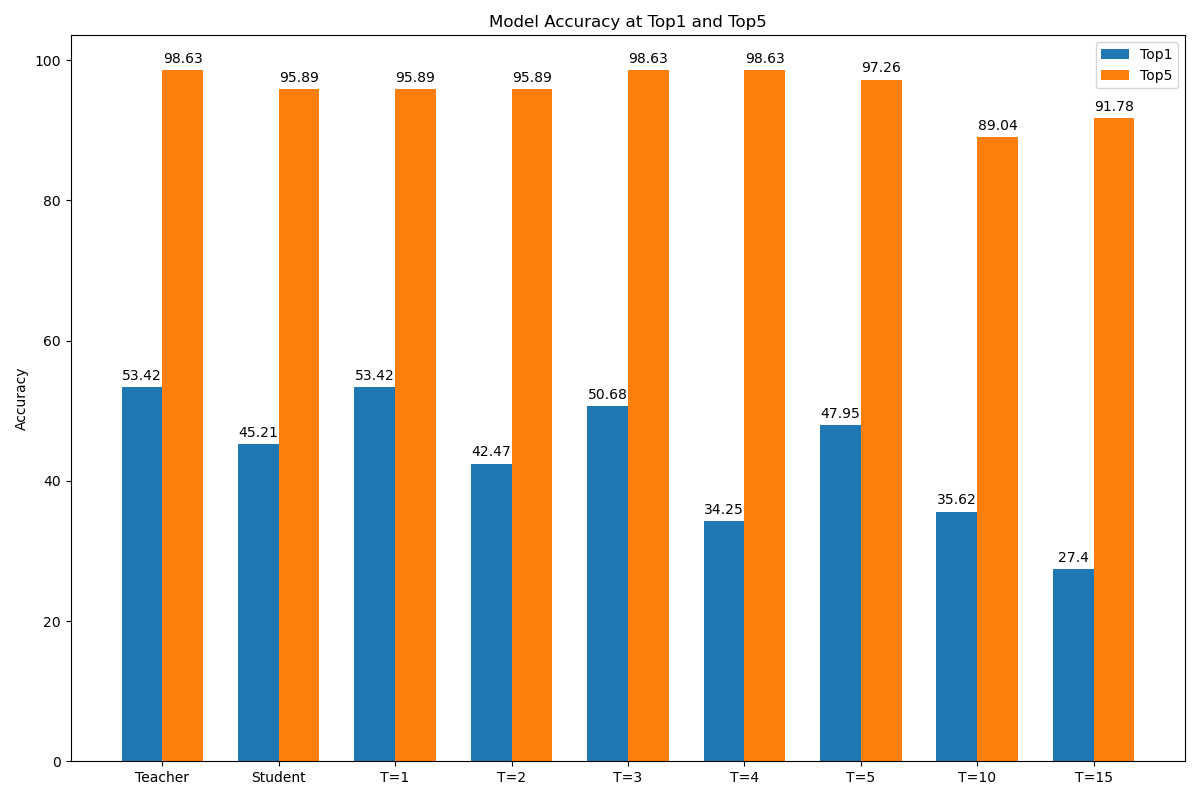
\includegraphics[width = \linewidth]{Top1 and Top5 Accuracy.png}
    \centering
    \caption{Accuratezze Top-1 e Top-5 di tutti i modelli impiegati per la Knowledge Distillation, ad una temperatura T variabile.}
    \label{accuracy_KD}
\end{figure}
%tabella accuratezze
\begin{table}
    \centering
    \begin{adjustbox}{max width=\textwidth}
    \begin{tabular}{|c||L|L||L|L|}
        \hline
        \multirow{2}{*}{\bfseries{MODELLI}} & \multicolumn{2}{c||}{\bfseries{IPER-PARAMETRI}} & \multicolumn{2}{c|}{\bfseries{ACCURATEZZA}}\\  & \bfseries{$\alpha$} & \bfseries{T}  & \bfseries{TOP-1} & \bfseries{TOP-5} \\
        \hline
        \hline
        {\bfseries{Insegnante}} & 1 & / & \color{blue}{\bfseries{53.42}} & \color{blue}{\bfseries{98.63}}\\
        \hline
        {\bfseries{Studente base}} & 0.25 & / & \color{blue}{\bfseries{45.21}} & \color{blue}{\bfseries{95.89}}\\
        \hline 
        {\bfseries{Studente-Dst}} & 0.25 & 1 & \color{red}53.42 & \color{red}95.89\\
        \hline
        {\bfseries{Studente-Dst}} & 0.25 & 2 & \color{red}42.47 & \color{red}95.89\\
        \hline
        {\bfseries{Studente-Dst}} & 0.25 & 3 & \color{green}{\bfseries{50.68}} & \color{green}{\bfseries{98.63}}\\
        \hline
        {\bfseries{Studente-Dst}} & 0.25 & 4 & \color{red}34.25 & \color{red}98.63\\
        \hline
        {\bfseries{Studente-Dst}} & 0.25 & 5 & \color{red}47.95 & \color{red}97.26\\
        \hline
        {\bfseries{Studente-Dst}} & 0.25 & 10 & \color{red}35.62 & \color{red}89.04\\
        \hline
        {\bfseries{Studente-Dst}} & 0.25 & 15 & \color{red}27.4 & \color{red}91.78\\
        \hline
    \end{tabular}
    \end{adjustbox}
    \vspace{0.5cm}
    \caption{Accuratezze Top-1 e Top-5 dei modelli Insengante, Studente base e Studente distillato (Dst) a diverse temperature T. I valori in blu sono le accuratezze di riferimento, mentre quei verdi rappresentano l'accuratezza dal modello scelto.}
    \label{accuracy_models_dist}
\end{table}


Per dimostrare la veridicità di tali accuratezze, sono state riportate in un grafico le curve di apprendimento di ogni modello ricavate dal numero di errori commessi, in fase di validazione, in ogni epoca (Fig \ref{lc_KD}).
\begin{figure}
    \centering
    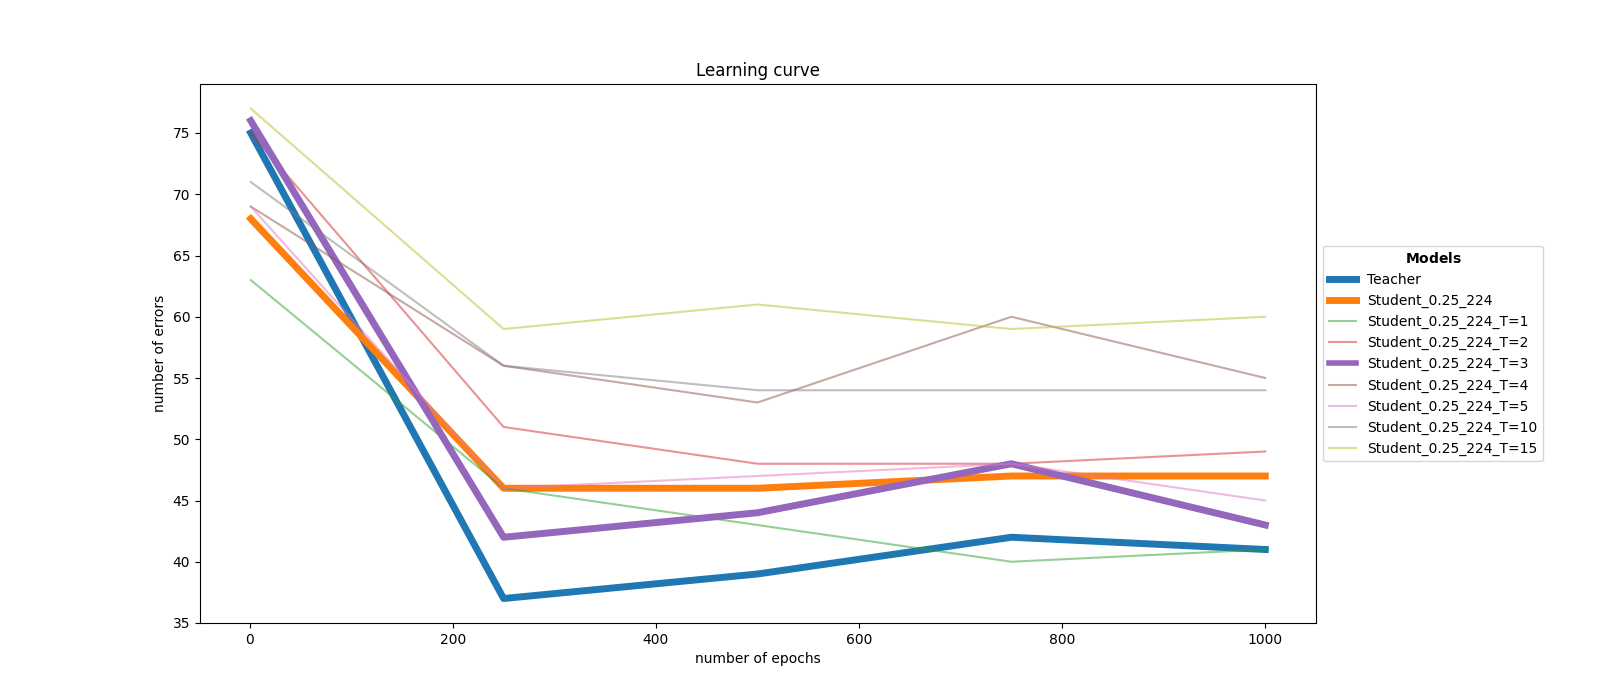
\includegraphics[width = 1.5\linewidth, angle=90, origin=c]{learning_curve KD.png}
    \centering
    \caption{Curva di apprendimento dei modelli impiegati per la Knowledge Distillation.}
    \label{lc_KD}
\end{figure}
Il grafico dimostra come la scelta del modello studente distillato, ad una temperatura T=3, vada ad interporsi tra le curve di apprendimento dell'insegnante e quelle dello studente base. Tale convergenza (linea viola) sta a significare che il modello studente distillato ha appreso la conoscenza trasmessa dall'insegnante (linea blu), discostandosi al contempo dal modello studente base (linea arancione) il quale non ha ricevuto alcun tipo di conoscenza. Il modello selezionato costituirà la rete base nell'architettura Single-Shot-Detector (SSD). 

\section{Riduzione numero di parametri}
Allo stato dell'arte esistono numerosi modelli deep learning che soffrono di una problematica comune: la numerosità dei parametri. Non è sempre vero che un gran numero dei parametri porti all'aumento dell'accuratezza di un modello. Questo problema non solo comporta maggior occupazione di memoria, ma ricade anche sulle prestazioni del modello, in termini di velocità di inferenza, e sul consumo energetico. In quest'ultimo caso, essendo circondati da dispostivi mobili con a bordo una batteria, difficilmente i modelli di grandi dimensioni troveranno un'implementazione. Questa rappresenta un'altra motivazione che ha consentito l'evoluzione delle tecniche di compressione. Dato che nell'elaborato vengono utilizzate due di queste tecniche, di seguito vengono mostrati i risultati inerenti la riduzione del numero di parametri sui modelli utilizzati.
\subsection{Riduzione via Pruning}
I grafici presenti nella sezione precedente, inerenti all'applicazione della tecnica di pruning su un modello SSD, hanno evidenziato come la maggior parte dei parametri utilizzati sia del tutto insignificante. Il modello SSD ha un quantità di parametri pari a $\sim{7.64}$ milioni. Prendendo in riferimento la tecnica di Unstructured pruning, i risultati ottenuti precedentemente dimostrano come il 40\% dei pesi possa essere eliminato senza influire sull'accuratezza del modello. Per un tasso di sparsità variabile tra 0 (pesi tutti azzerati) e 100 (pesi tutti diversi da zero), viene riportata in Figura \ref{par_pruning} l'ammontare del numero di parametri allenabili, e quindi diversi da zero, del modello SSD.
Tenendo in considerazione la soglia del 40\% di sparsità, la struttura del modello si ritroverebbe con $\sim{3.04}$ milioni di pesi in meno, giungendo quindi a una quantità totale di $\sim{4.60}$ milioni di parametri. La significativa riduzione non può altro che rappresentare un beneficio per i dispositivi con i limiti precedentemente descritti.
\begin{figure}
    \centering
    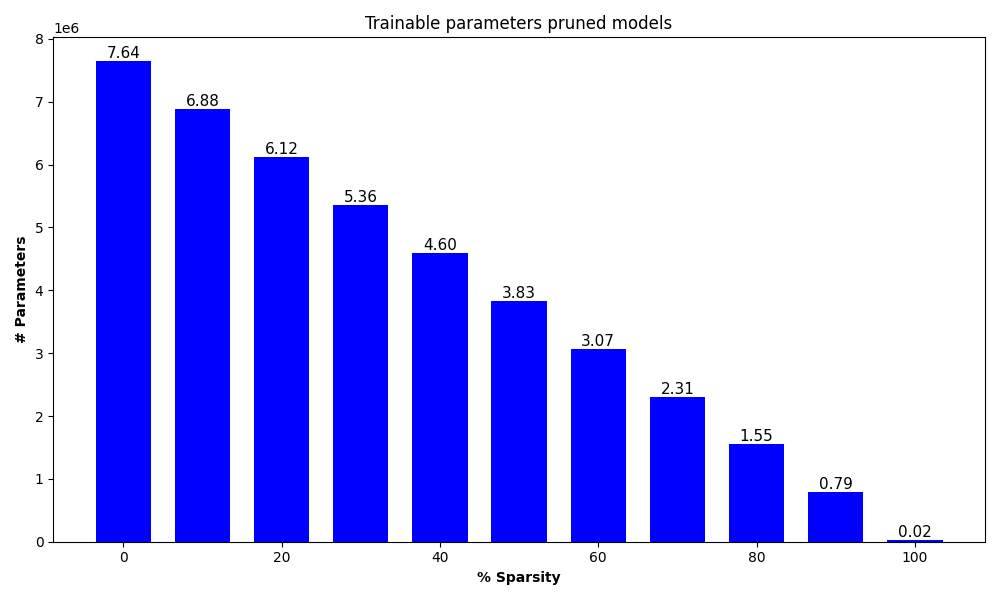
\includegraphics[width = \linewidth]{Pruning_Unstructured_parameters.png}
    \centering
    \caption{Riduzione del numero di parametri via pruning a sparistà variabile.}
    \label{par_pruning}
\end{figure}
\subsection{Riduzione via Knowledge Distillation}\index{Knowledge Distillation}
Al fine di verificare la veridicità della tecnica di Knowledge distillation, premeva la necessità di costruire un modello studente di dimensioni più piccole rispetto al modello insegnante. I meriti per la realizzazione di questa fase non sono da attribuirsi alla tecnica di compressione in questione, ma vanno dati agli autori della rete MobileNet-V1 grazie all'implementazione del parametro width multiplier.
Impostando  ($\alpha=0.25$) la rete studente ha avuto un decremento pari al 93,31\% dei parametri rispetto all'insegnante. Avendo quest'ultimo un numero di parametri maggiore di 3 milioni, il nuovo modello studente si ritrova con $\sim{200}$ mila parametri allenabili (Fig. \ref{base_net_par}).
\begin{figure}
    \centering
    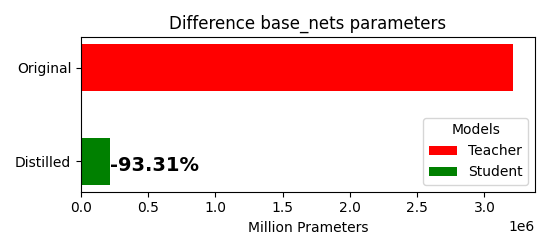
\includegraphics[width = 0.9\linewidth]{Difference base_nets parameters.png}
    \centering
    \caption{Riduzione del numero di parametri del modello base via Knowledge distillation.}
    \label{base_net_par}
\end{figure}
Per quanto riguarda l'intera rete DSSD, composta dalla rete base dello studente distillato e dalla restante parte di livelli convoluzionali a dimensioni ridotte, è stato possibile raggiungere una significativa diminuzione del numero di parametri. Ricordando che il modello insegnante ha un numero di parametri di $\sim{7.64}$ milioni, il modello DSSD proposto raggiunge poco più di $\sim{850}$ mila parametri (Fig. \ref{SSD_par}), discostandosi quindi di una quantità significativa.
\begin{figure}
    \centering
    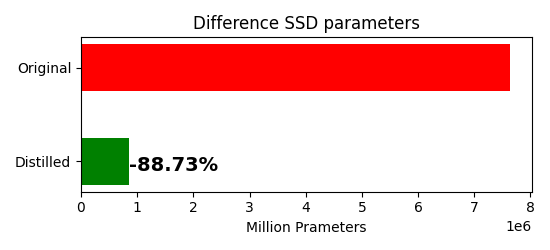
\includegraphics[width = 0.9\linewidth]{Difference SSD parameters.png}
    \centering
    \caption{Riduzione del numero di parametri del modello proposto DSSD via Knowledge distillation.}
    \label{SSD_par}
\end{figure}

\section{Riduzione della dimesione occupata}
Le tecniche di compressione studiate si sono rivelate utili per poter ridurre il numero di parametri all'interno di un modello. Una tale riduzione comporta, a sua volta, un risparmio sull'occupazione della memoria. Oltre che a rappresentare un beneficio per la memoria, a gioire sono i piccoli dispositivi, come per esempio gli indossabili (es: smartwatch), o tutti quei sistemi embedded, la cui disponibilità di memoria rappresenta un punto cruciale per l'ottimizzazione dei vari processi. Il raggiungimento di questo obiettivo permette anche risparmiare anche le risorse energetiche  per la gestione del modello. Passando al concreto, le due tecniche di compressione studiate permetto di raggiungere tale scopo. Seguono delle sezioni contenenti tutti i risultati ottenuti.
\subsection{Dimensione risultante dal Pruning}
I modelli ricavati da una tecnica di pruning hanno un numero di parametri minore rispetto al modello sorgente. Purtroppo, attualmente sono pochi i benefici che possono essere sfruttati quando a comprimere un modello sono dei framework incapaci di rimuovere alcun tipo di parametro superfluo. L'unico vantaggio ricercato, riguarda la sottomissione di tali modelli agli algoritmi presenti nei software di compressione (es: gzip). Un tale programma sarebbe in grado di ottimizzare le dimensioni di un file quando questo è composto da numerosi zeri. Prendendo sempre in riferimento il modello SSD, la sua compressione porterebbe alla creazione di un file di dimensioni uguali a 28.8 MB (Fig. \ref{SSD_dim}). Già in questa prima compressione vi è una riduzione delle dimensioni originali pari al 6\%. Se la soglia scelta resta ancora quella del 40\% di sparsità, allora le dimensioni si ridurrebbero a 19.4 MB, per un totale pari al 36\% di riduzione. Tale quantità risparmiata rappresenta un enorme beneficio per i dispositivi a memoria limitata.
\begin{figure}
    \centering
    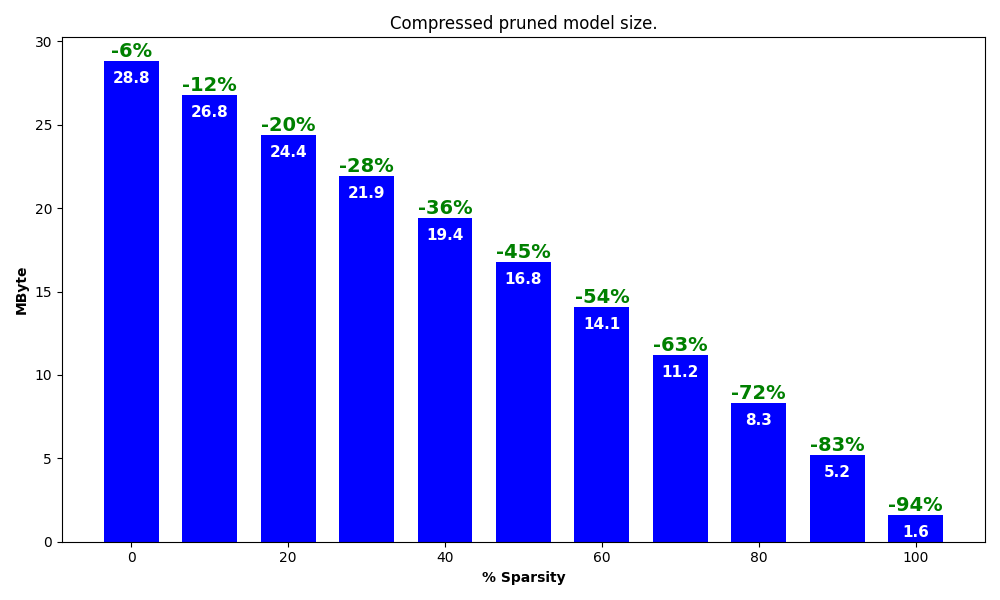
\includegraphics[width = \linewidth]{Unstructured_size_reduction.png}
    \centering
    \caption{Riduzione della dimensione del modello SSD via pruning.}
    \label{SSD_dim}
\end{figure}

\subsection{Dimensione risultante dalla Knowledge Distillation}\index{Knowledge Distillation}
Dalla riduzione del numero di parametri raggiunta sul modello base, nonché il modello studente distillato, la quantità di memoria risparmiata è davvero significante. Data la notevole dimensione del modello insegnante, si è cercato di ridurre anche la dimensione della sua sottorete  (backbone), rendendola nel complesso più leggera e più veloce dal punto di vista computazionale. Presa singolarmente, la sottorete MobileNet-V1 originale ha una dimensione maggiore ai 12MB. Il modello base studente distillato, è stato in grado di raggiungere una dimensione inferiore del 92.71\%, affiancandosi ad una dimensione leggermente inferiore a 1 MB (Fig. \ref{base_dim}).
\begin{figure}
    \centering
    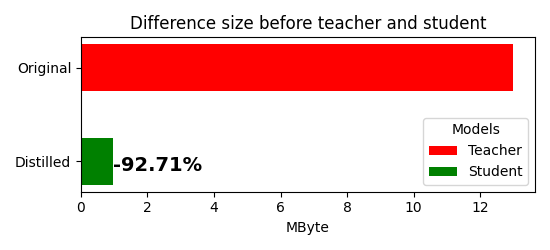
\includegraphics[width = 0.9\linewidth]{Different size base_net.png}
    \centering
    \caption{Riduzione della dimensione del modello base via Knowledge distillation.}
    \label{base_dim}
\end{figure}
Volendo calcolare la dimensione dell'intera rete DSSD, dopo aver modificato le dimensioni della restante parte formata dai livelli convoluzionali, la dimensione totale raggiunta è inferiore dell'88.60\% rispetto alla rete SSD originale. Rappresentando entrami i modelli sotto forma di dimensioni occupate, l'intero modello SSD occupa 30.7MB contro i 3.4MB del modello DSSD (Fig. \ref{SSD_dim_KD}). E con estrema fermezza, si può confermare che un obiettivo essenziale dell'elaborato è stato portato a termine.
\begin{figure}
    \centering
    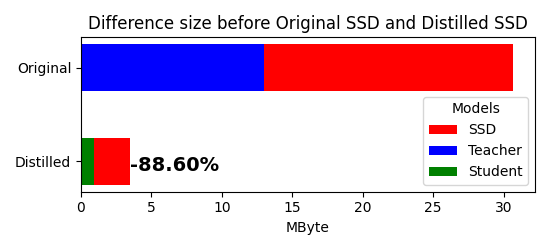
\includegraphics[width = 0.9\linewidth]{Different size SSD.png}
    \centering
    \caption{Riduzione della dimensione del modello SSD via Knowledge distillation.}
    \label{SSD_dim_KD}
\end{figure}

\section{Benchmarks}
Sin dall'inizio, l'obiettivo principale da raggiungere riguardava lo sviluppo di un modello in grado di superare i limiti dei modelli pre-addestrati, ottenendo una di velocità di elaborazione maggiore. Per adempire a questo scopo, bisogna ricavare prima le performance dei modelli pre-addestrati, in modo da avere una base di riferimento costituente il punto di partenza.
Al fine di capire le potenzialità messe a disposizione dalle varie architetture di riferimento, di seguito vengono riportati dei benchmarks riguardanti la comparazione dei Frame-per-Second (FPS) raggiunti, in fase di inferenza, da ciascuna macchina.
In ogni dataset esistono diversi set di immagini, ognuno con diversa risoluzione. Per quanto riguarda l'inferenza, l'input sottoposto ad ogni modello proviene da sei diversi video (.mp4) e dallo streaming di due webcam, tutti aventi diversa risoluzione e numero di FPS (Tab. (\ref{source})). Nelle tabelle seguenti, contenenti i valori ricavati dai test, sono presenti due tipologie di campi, maggiormente discussi nel capitolo precedente:
\begin{itemize}
    \item {\bfseries{\emph{Out}}}: indica il numero di FPS visualizzabili a schermo;
    \item {\bfseries{\emph{Net}}}: indica il numero di FPS elaborati da una specifica rete durante l'inferenza.
\end{itemize}

\begin{table}
    \renewcommand{\baselinestretch}{1}
    \centering
    \begin{adjustbox}{max width=\textwidth}
    \begin{tabular}{|c||c|c||}
        \hline
        \multirow{2}{*}{\bfseries{Sorgente}} & \multicolumn{2}{c||}{\bfseries{Specifiche Input}}\\            & \bfseries{Qualità} & \bfseries{FPS}\\
        \hline
        \hline
        \RN{1} Video & 240p & 60\\
        \hline
        \RN{2} Video & 360p & 30\\
        \hline 
        \RN{3} Video & 480p & 30\\
        \hline
        \RN{4} Video & 720p &  30\\
        \hline
        \RN{5} Video & 1080p & 30\\
        \hline
        \RN{6} Video & 1080p & 60\\
        \hline
        \RN{7} Webcam1 & 720p & 30\\
        \hline
        \RN{8} Webcam2 & 1080p & 30\\
        \hline
    \end{tabular}
    \end{adjustbox}
    \vspace{0.5cm}
    \caption{Specifiche sorgenti input.}
    \label{source}
\end{table}

\subsection{Perfomance modelli pre-addestrati}
I primi risultati ottenuti riguardano le performance raggiunte, in fase di inferenza, dai modelli pre-addestrati. I valori ricavati rappresentano il limite minimo da raggiungere da parte del modello proposto DSSD. Le tre architetture di riferimento hanno permesso di ottenere le performance descritte nei sotto-paragrafi successivi.

\subsubsection{Benchmarks Jetson Nano}
I test effettuati sulla scheda Jetson Nano, sono stati eseguiti utilizzando i framework ampiamente descritti nella sezione \ref{acceleratori}.
Per ottenere una comparazione tra i due acceleratori, vengono effettuati due benchmarks distinti, uno per l'attività di object detection e il secondo per l'attività di semantic segmentation.
Ricapitolando, le librerie sviluppate interamente da NVidia, permettono l'ottimizzazione delle performance dei sistemi embedded appartenenti alla famiglia Jetson. L'efficienza di questo set di librerie proviene dall'utilizzo dell'SDK TensorRT, utile ad offrire una bassa latenza e un throughtput elevato per inferenze deep learning ad alte prestazioni. Tutte le applicazioni basate su TensorRT raggiungono delle prestazioni fino a 40 volte più veloci rispetto alle piattaforme dotate di sola CPU. Solo le macchine provviste di schede grafiche NVidia possono godere di tale beneficio. A bordo di queste è presente la tecnologia CUDA, un modello di programmazione parallela specializzato nell'ottimizzazione dell'inferenza che si avvale di librerie e strumenti di sviluppo fondate su CUDA-X. Quest'ultime sono molto utilizzate  in ambiti di intelligenza artificiale, guida autonoma, elaborazioni ad alte prestazioni e gestione della grafica. 
I benchmarks svolti con il supporto di queste librerie, riguardano le attività di object detection (Tab. \ref{obj_jetson_utils}) e semantic segmentation (Tab. \ref{sem_seg_jetson_utils}).
Per la loro formazione, i modelli pre-addestrati sulla tecnica di semantic segmentation hanno utilizzato le immagini contenute nei dataset Cityscapes e Pascal Voc. Per quanto riguarda invece i modelli pre-addestrati nell'attività di object detection, questi si sono serviti delle immagini presenti nei restanti datasets descritti nella sezione \ref{datasets_description}.
Per un dispositivo embedded di fascia economica, questi risultati rappresentano delle performance promettenti rispetto alla concorrenza.
Le performance ottenute con OpenCV tramite l'utilizzo dell'acceleratore cuDNN sono visibili nella Tabella \ref{sem_seg_jetson_utils_opencv_gpu}, mentre in Tabella \ref{sem_seg_jetson_utils_opencv_cpu} vengono riportate le performance riguardanti l'inferenza avvenuta sulla CPU.
Confrontando i risultati ottenuti con le jetson.utils, si evince che l'assenza di un ottimizzatore ad hoc, porti l'intero sistema a raggiungere delle performance inferiori.
Per verificare la veridicità dei benchmarks effettuati con le jetson utils, è possibile svolgere una comparazione con i risultati dichiarati direttamente dal produttore \cite{performance_obj_det_jetson}.
Per entrambe le attività, nelle tabelle (\ref{average performance jetson utils obj_det}) e (\ref{average performance jetson utils sem_seg}) vengono riportate le medie degli FPS ricavate dall'utilizzo delle jetson utils, mentre nelle Tabelle (\ref{average performance jetson opencv GPU sem_seg}) e (\ref{average performance jetson opencv CPU sem_seg})  vengono riportati i corrispettivi valori medi raggiunti utilizzando OpenCV.

\begin{table}
    \renewcommand{\baselinestretch}{1}
    \centering
    \begin{adjustbox}{max width=\textwidth}
    \begin{tabular}{|c||c|c||c|c||}
        \hline
        \multirow{2}{*}{\bfseries{\Large Modelli}} & \multicolumn{2}{c||}{\bfseries{30 FPS}} & \multicolumn{2}{c||}{\bfseries{60 FPS}}\\            & \bfseries{Output} & \bfseries{Network} & \bfseries{Output} & \bfseries{Network}\\
        \hline
        \hline
        SSD-MOBILENET-V1 & 15.93 & 34.23 & 15.24 & 34.84\\
        \hline
        SSD-MOBILENET-V2 & 14.29 & 27.04 & 13,66 & 27.19\\
        \hline 
        SSD-INCEPTION-V2 & 12.65 & 21.68 & 11.85 & 21.7\\
        \hline
        PEDNET & 6.83 &  8.91 & 6.73 & 8.92\\
        \hline
        MULTIPEDNET & 6.84 & 9.11 & 6.81 & 9.12\\
        \hline
    \end{tabular}
    \end{adjustbox}
    \vspace{0.5cm}
    \caption{Performance FPS medi nell'attività di Object Detection su Jetson Nano (\emph{utils}).}
    \label{average performance jetson utils obj_det}
\end{table}

\begin{table}
    \renewcommand{\baselinestretch}{1}
    \centering
    \begin{adjustbox}{max width=\textwidth}
    \begin{tabular}{|c||c|c||c|c||}
        \hline
        \multirow{2}{*}{\bfseries{\Large Modelli-Dataset}} & \multicolumn{2}{c||}{\bfseries{30 FPS}} & \multicolumn{2}{c||}{\bfseries{60 FPS}}\\            & \bfseries{Output} & \bfseries{Network} & \bfseries{Output} & \bfseries{Network}\\
        \hline
        \hline
        RN18-CS (512x256) & 10.43 & 48.51 & 12.56 & 48.5\\
        \hline
        RN18-CS (1024x512) & 6.01 & 12.29 & 6.09 & 12.32\\
        \hline 
        RN18-CS (2048x1024) & 3,13 & 3,05 & 3.1 & 3.04\\
        \hline
        RN18-VOC (320x320) & 10.19 &  46.31 & 12.57 & 46.20\\
        \hline
        RN18-VOC (512x320) & 9.30 & 34.45 & 10.94 & 34.39\\
        \hline
    \end{tabular}
    \end{adjustbox}
    \vspace{0.5cm}
    \caption{Performance FPS medi nell'attività di Semantic Segmentation Jetson Nano (\emph{utils}).}
    \label{average performance jetson utils sem_seg}
\end{table}

\begin{table}
    \renewcommand{\baselinestretch}{1}
    \centering
    \begin{adjustbox}{max width=\textwidth}
    \begin{tabular}{|c||c|c||c|c||}
        \hline
        \multirow{2}{*}{\bfseries{\Large Modelli-Dataset}} & \multicolumn{2}{c||}{\bfseries{30 FPS}} & \multicolumn{2}{c||}{\bfseries{60 FPS}}\\            & \bfseries{Output} & \bfseries{Network} & \bfseries{Output} & \bfseries{Network}\\
        \hline
        \hline
        RN18-CS (512x256) & 8.03 & 19.45 & 10.66 & 19.58\\
        \hline
        RN18-CS (1024x512) & 3.52 & 5.11 & 3.94 & 5.37\\
        \hline 
        RN18-CS (2048x1024) & 1.20 & 1.45 & 1,17 & 1.46\\
        \hline
        RN18-VOC (320x320) & 7.68 &  17.53 & 10.11 & 17.7\\
        \hline
        RN18-VOC (512x320) & 6.89 & 14.87 & 8.7 & 14.96\\
        \hline
    \end{tabular}
    \end{adjustbox}
    \vspace{0.5cm}
    \caption{Performance FPS medi nell'attività di Semantic Segmentation Jetson Nano (\emph{OpenCV - GPU}).}
    \label{average performance jetson opencv GPU sem_seg}
\end{table}

\begin{table}
    \renewcommand{\baselinestretch}{1}
    \centering
    \begin{adjustbox}{max width=\textwidth}
    \begin{tabular}{|c||c|c||c|c||}
        \hline
        \multirow{2}{*}{\bfseries{\Large Modelli-Dataset}} & \multicolumn{2}{c||}{\bfseries{30 FPS}} & \multicolumn{2}{c||}{\bfseries{60 FPS}}\\            & \bfseries{Output} & \bfseries{Network} & \bfseries{Output} & \bfseries{Network}\\
        \hline
        \hline
        RN18-CS (512x256) & 1.46 & 1.61 & 1.49 & 1.63\\
        \hline
        RN18-CS (1024x512) & 0.37 & 0.38 & 0.39 & 0.4\\
        \hline 
        RN18-CS (2048x1024) & 0.09 & 0.09 & 0.09 & 0.09\\
        \hline
        RN18-VOC (320x320) & 1.85 &  2.07 & 1.89 & 2.14\\
        \hline
        RN18-VOC (512x320) & 1.22 & 1.32 & 1.25 & 1.36\\
        \hline
    \end{tabular}
    \end{adjustbox}
    \vspace{0.5cm}
    \caption{Performance FPS medi nell'attività di Semantic Segmentation Jetson Nano (\emph{OpenCV - CPU}).}
    \label{average performance jetson opencv CPU sem_seg}
\end{table}

\begin{landscape}
    \renewcommand{\baselinestretch}{1}
    \centering
    \begin{table}
        \newarray\First
        \newarray\Second
        \newarray\Third
        \newarray\Fourth
        \newarray\Fifth
        \readarray{First}{20&44.83&20.49&45.13&20.47&45.10&19.19&44.89&17.75&44.68&17.52&44.22&17.52&44.43&15.78&44.60}
        \readarray{Second}{15.74&27.31&14.38&27.39&16.24&27.22&15.57&27.07&15.12&26.41&13.93&27&11&27.06&11.09&27.17}
        \readarray{Third}{13.77&21.55&12.38&22&13.93&21.69&13.81&21.67&13.83&21.51&12.31&21.56&9.82&21.81&9.78&21.71}
        \readarray{Fourth}{7.02&8.92&6.83&8.94&6.87&8.93&6.89&8.92&6.91&8.87&6.81&8.89&6.52&8.93&6.6&8.91}
        \readarray{Fifth}{7.02&9.13&6.79&9.12&7.02&9.16&6.96&9.15&6.92&9.07&6.76&9.15&6.57&9.08&6.61&9.08}
        {\scriptsize %
        \begin{tabular}{|c||c|c||c|c||c|c||c|c||c|c||c|c||c|c||c|c||}
            \hline
            & \multicolumn{16}{c||}{ \multirow{3}{*}{\bfseries{\large OBJECT DETECTION (DETECTNET) - JETSON NANO (utils)}}}\\
            & \multicolumn{16}{c||}{}\\
            & \multicolumn{16}{c||}{}\\
            \hline
            \multirow{2}{*}{\bfseries{\large Modelli}} 
            & \multicolumn{2}{c||}{\bfseries{\normalsize Webcam1}} & \multicolumn{2}{c||}{\bfseries{\normalsize Webcam2}} & \multicolumn{2}{c||}{\bfseries{\normalsize \RN{1} Video}} & \multicolumn{2}{c||}{\bfseries{\normalsize \RN{2} Video}} & \multicolumn{2}{c||}{\bfseries{\normalsize \RN{3} Video}} & \multicolumn{2}{c||}{\bfseries{\normalsize \RN{4} Video}} & \multicolumn{2}{c||}{\bfseries{\normalsize \RN{5} Video}} & \multicolumn{2}{c||}{\bfseries{\normalsize \RN{6} Video}}\\            & \bfseries{\footnotesize Out} & \bfseries{\footnotesize Net} & \bfseries{\footnotesize Out} & \bfseries{\footnotesize Net} & \bfseries{\footnotesize Out} & \bfseries{\footnotesize Net} & \bfseries{\footnotesize Out} & \bfseries{\footnotesize Net} & \bfseries{\footnotesize Out} & \bfseries{\footnotesize Net} & \bfseries{\footnotesize Out} & \bfseries{\footnotesize Net} & \bfseries{\footnotesize Out} & \bfseries{\footnotesize Net} & \bfseries{\footnotesize Out} & \bfseries{\footnotesize Net}\\
            \hline
            \multirow{2}{*}{SSD-MOBILENET-V1} & \multirow{2}{*}{\First(1)} & \multirow{2}{*}{\First(2)} & \multirow{2}{*}{\First(3)} & \multirow{2}{*}{\First(4)} & \multirow{2}{*}{\First(5)} & \multirow{2}{*}{\First(6)} & \multirow{2}{*}{\First(7)} & \multirow{2}{*}{\First(8)} & \multirow{2}{*}{\First(9)} & \multirow{2}{*}{\First(10)} & \multirow{2}{*}{\First(11)} & \multirow{2}{*}{\First(12)} & \multirow{2}{*}{\First(13)} & \multirow{2}{*}{\First(14)} & \multirow{2}{*}{\First(15)} & \multirow{2}{*}{\First(16)}\\
            & & & & & & & & & & & & & & & &\\
            \hline
            \multirow{2}{*}{SSD-MOBILENET-V2}& \multirow{2}{*}{\Second(1)} & \multirow{2}{*}{\Second(2)} & \multirow{2}{*}{\Second(3)} & \multirow{2}{*}{\Second(4)} & \multirow{2}{*}{\Second(5)} & \multirow{2}{*}{\Second(6)} & \multirow{2}{*}{\Second(7)} & \multirow{2}{*}{\Second(8)} & \multirow{2}{*}{\Second(9)} & \multirow{2}{*}{\Second(10)} & \multirow{2}{*}{\Second(11)} & \multirow{2}{*}{\Second(12)} & \multirow{2}{*}{\Second(13)} & \multirow{2}{*}{\Second(14)} & \multirow{2}{*}{\Second(15)} & \multirow{2}{*}{\Second(16)}\\
            & & & & & & & & & & & & & & & &\\
            \hline 
            \multirow{2}{*}{SSD-INCEPTION-V2}& \multirow{2}{*}{\Third(1)} & \multirow{2}{*}{\Third(2)} & \multirow{2}{*}{\Third(3)} & \multirow{2}{*}{\Third(4)} & \multirow{2}{*}{\Third(5)} & \multirow{2}{*}{\Third(6)} & \multirow{2}{*}{\Third(7)} & \multirow{2}{*}{\Third(8)} & \multirow{2}{*}{\Third(9)} & \multirow{2}{*}{\Third(10)} & \multirow{2}{*}{\Third(11)} & \multirow{2}{*}{\Third(12)} & \multirow{2}{*}{\Third(13)} & \multirow{2}{*}{\Third(14)} & \multirow{2}{*}{\Third(15)} & \multirow{2}{*}{\Third(16)}\\
            & & & & & & & & & & & & & & & &\\
            \hline
            \multirow{2}{*}{PEDNET}& \multirow{2}{*}{\Fourth(1)} & \multirow{2}{*}{\Fourth(2)} & \multirow{2}{*}{\Fourth(3)} & \multirow{2}{*}{\Fourth(4)} & \multirow{2}{*}{\Fourth(5)} & \multirow{2}{*}{\Fourth(6)} & \multirow{2}{*}{\Fourth(7)} & \multirow{2}{*}{\Fourth(8)} & \multirow{2}{*}{\Fourth(9)} & \multirow{2}{*}{\Fourth(10)} & \multirow{2}{*}{\Fourth(11)} & \multirow{2}{*}{\Fourth(12)} & \multirow{2}{*}{\Fourth(13)} & \multirow{2}{*}{\Fourth(14)} & \multirow{2}{*}{\Fourth(15)} & \multirow{2}{*}{\Fourth(16)}\\
            & & & & & & & & & & & & & & & &\\
            \hline
            \multirow{2}{*}{MULTIPEDNET}& \multirow{2}{*}{\Fifth(1)} & \multirow{2}{*}{\Fifth(2)} & \multirow{2}{*}{\Fifth(3)} & \multirow{2}{*}{\Fifth(4)} & \multirow{2}{*}{\Fifth(5)} & \multirow{2}{*}{\Fifth(6)} & \multirow{2}{*}{\Fifth(7)} & \multirow{2}{*}{\Fifth(8)} & \multirow{2}{*}{\Fifth(9)} & \multirow{2}{*}{\Fifth(10)} & \multirow{2}{*}{\Fifth(11)} & \multirow{2}{*}{\Fifth(12)} & \multirow{2}{*}{\Fifth(13)} & \multirow{2}{*}{\Fifth(14)} & \multirow{2}{*}{\Fifth(15)} & \multirow{2}{*}{\Fifth(16)}\\
            & & & & & & & & & & & & & & & &\\
            \hline
        \end{tabular}
        }%
        \vspace{0.2cm}
        \caption{FPS Performance nell'attività di Object Detection su Jetson Nano (\emph{utils}).}
        \label{obj_jetson_utils}
    \end{table}

    \begin{table}
        \newarray\Firsts
        \newarray\Second
        \newarray\Third
        \newarray\Fourth
        \newarray\Fifth
        \readarray{Firsts}{8.25&48.12&8.37&48.94&20.49&48.92&16.68&48.75&15.7&48.6&9.19&48.24&4.43&48.42&4.63&48.08}
        \readarray{Second}{5.76&12.27&5.57&12.35&8.22&12.34&7.38&12.27&7.46&12.34&5.46&12.3&4.43&12.21&3.96&12.31}
        \readarray{Third}{3.79&3.04&2.56&3.06&4.41&3.06&2.38&3.06&4.31&3.06&2.17&3.06&3.58&3.06&1.79&3.02}
        \readarray{Fourth}{8.96&46.06&7.9&46.44&20.19&46.43&16.37&46.46&15.32&46.63&7.82&46.26&4.78&46.03&4.96&45.98}
        \readarray{Fifth}{8.4&34.31&8.15&34.92&17.15&34.35&13.52&34.26&13.82&34.43&7.42&34.21&4.5&34.61&4.74&34.44}
        {\scriptsize %
        \begin{tabular}{|c||c|c||c|c||c|c||c|c||c|c||c|c||c|c||c|c||}
            \hline
            & \multicolumn{16}{c||}{ \multirow{3}{*}{\bfseries{\large SEMANTIC SEGMENTATION (SEGNET) - JETSON NANO (utils)}}}\\
            & \multicolumn{16}{c||}{}\\
            & \multicolumn{16}{c||}{}\\
            \hline
            \multirow{2}{*}{\bfseries{\large Modelli-Dati}} 
            & \multicolumn{2}{c||}{\bfseries{\normalsize Webcam1}} & \multicolumn{2}{c||}{\bfseries{\normalsize Webcam2}} & \multicolumn{2}{c||}{\bfseries{\normalsize \RN{1} Video}} & \multicolumn{2}{c||}{\bfseries{\normalsize \RN{2} Video}} & \multicolumn{2}{c||}{\bfseries{\normalsize \RN{3} Video}} & \multicolumn{2}{c||}{\bfseries{\normalsize \RN{4} Video}} & \multicolumn{2}{c||}{\bfseries{\normalsize \RN{5} Video}} & \multicolumn{2}{c||}{\bfseries{\normalsize \RN{6} Video}}\\            & \bfseries{\footnotesize Out} & \bfseries{\footnotesize Net} & \bfseries{\footnotesize Out} & \bfseries{\footnotesize Net} & \bfseries{\footnotesize Out} & \bfseries{\footnotesize Net} & \bfseries{\footnotesize Out} & \bfseries{\footnotesize Net} & \bfseries{\footnotesize Out} & \bfseries{\footnotesize Net} & \bfseries{\footnotesize Out} & \bfseries{\footnotesize Net} & \bfseries{\footnotesize Out} & \bfseries{\footnotesize Net} & \bfseries{\footnotesize Out} & \bfseries{\footnotesize Net}\\
            \hline
            \multirow{2}{*}{RN18-CS (512x256)} & \multirow{2}{*}{\Firsts(1)} & \multirow{2}{*}{\Firsts(2)} & \multirow{2}{*}{\Firsts(3)} & \multirow{2}{*}{\Firsts(4)} & \multirow{2}{*}{\Firsts(5)} & \multirow{2}{*}{\Firsts(6)} & \multirow{2}{*}{\Firsts(7)} & \multirow{2}{*}{\Firsts(8)} & \multirow{2}{*}{\Firsts(9)} & \multirow{2}{*}{\Firsts(10)} & \multirow{2}{*}{\Firsts(11)} & \multirow{2}{*}{\Firsts(12)} & \multirow{2}{*}{\Firsts(13)} & \multirow{2}{*}{\Firsts(14)} & \multirow{2}{*}{\Firsts(15)} & \multirow{2}{*}{\Firsts(16)}\\
            & & & & & & & & & & & & & & & &\\
            \hline
            \multirow{2}{*}{RN18-CS (1024x512)}& \multirow{2}{*}{\Second(1)} & \multirow{2}{*}{\Second(2)} & \multirow{2}{*}{\Second(3)} & \multirow{2}{*}{\Second(4)} & \multirow{2}{*}{\Second(5)} & \multirow{2}{*}{\Second(6)} & \multirow{2}{*}{\Second(7)} & \multirow{2}{*}{\Second(8)} & \multirow{2}{*}{\Second(9)} & \multirow{2}{*}{\Second(10)} & \multirow{2}{*}{\Second(11)} & \multirow{2}{*}{\Second(12)} & \multirow{2}{*}{\Second(13)} & \multirow{2}{*}{\Second(14)} & \multirow{2}{*}{\Second(15)} & \multirow{2}{*}{\Second(16)}\\
            & & & & & & & & & & & & & & & &\\
            \hline 
            \multirow{2}{*}{RN18-CS (2048x1024)}& \multirow{2}{*}{\Third(1)} & \multirow{2}{*}{\Third(2)} & \multirow{2}{*}{\Third(3)} & \multirow{2}{*}{\Third(4)} & \multirow{2}{*}{\Third(5)} & \multirow{2}{*}{\Third(6)} & \multirow{2}{*}{\Third(7)} & \multirow{2}{*}{\Third(8)} & \multirow{2}{*}{\Third(9)} & \multirow{2}{*}{\Third(10)} & \multirow{2}{*}{\Third(11)} & \multirow{2}{*}{\Third(12)} & \multirow{2}{*}{\Third(13)} & \multirow{2}{*}{\Third(14)} & \multirow{2}{*}{\Third(15)} & \multirow{2}{*}{\Third(16)}\\
            & & & & & & & & & & & & & & & &\\
            \hline
            \multirow{2}{*}{RN18-VOC (320x320)}& \multirow{2}{*}{\Fourth(1)} & \multirow{2}{*}{\Fourth(2)} & \multirow{2}{*}{\Fourth(3)} & \multirow{2}{*}{\Fourth(4)} & \multirow{2}{*}{\Fourth(5)} & \multirow{2}{*}{\Fourth(6)} & \multirow{2}{*}{\Fourth(7)} & \multirow{2}{*}{\Fourth(8)} & \multirow{2}{*}{\Fourth(9)} & \multirow{2}{*}{\Fourth(10)} & \multirow{2}{*}{\Fourth(11)} & \multirow{2}{*}{\Fourth(12)} & \multirow{2}{*}{\Fourth(13)} & \multirow{2}{*}{\Fourth(14)} & \multirow{2}{*}{\Fourth(15)} & \multirow{2}{*}{\Fourth(16)}\\
            & & & & & & & & & & & & & & & &\\
            \hline
            \multirow{2}{*}{RN18-VOC (512x320)}& \multirow{2}{*}{\Fifth(1)} & \multirow{2}{*}{\Fifth(2)} & \multirow{2}{*}{\Fifth(3)} & \multirow{2}{*}{\Fifth(4)} & \multirow{2}{*}{\Fifth(5)} & \multirow{2}{*}{\Fifth(6)} & \multirow{2}{*}{\Fifth(7)} & \multirow{2}{*}{\Fifth(8)} & \multirow{2}{*}{\Fifth(9)} & \multirow{2}{*}{\Fifth(10)} & \multirow{2}{*}{\Fifth(11)} & \multirow{2}{*}{\Fifth(12)} & \multirow{2}{*}{\Fifth(13)} & \multirow{2}{*}{\Fifth(14)} & \multirow{2}{*}{\Fifth(15)} & \multirow{2}{*}{\Fifth(16)}\\
            & & & & & & & & & & & & & & & &\\
            \hline
        \end{tabular}
        }%
        \vspace{0.2cm}
        \caption{FPS Performance nell'attività di Semantic Segmentation su Jetson Nano (\emph{utils}).}
        \label{sem_seg_jetson_utils}
    \end{table}
\end{landscape}

\begin{landscape}
    \renewcommand{\baselinestretch}{1}
    \centering
    \begin{table}
        \newarray\Firsts
        \newarray\Second
        \newarray\Third
        \newarray\Fourth
        \newarray\Fifth
        \readarray{Firsts}{6.19&18.93&2&19.63&16.41&19.81&14.27&19.69&14.24&19.7&6.62&19.53&4.88&19.24&4.91&19.35}
        \readarray{Second}{3.4&4.99&2&5.53&5.02&5.39&4.75&5.2&4.76&5.2&3.38&4.77&2.86&4.99&2.86&5.36}
        \readarray{Third}{1.09&1.44&1.24&1.45&1.34&1.46&1.34&1.46&1.31&1.46&1.23&1.45&1&1.46&1&1.46}
        \readarray{Fourth}{6.02&17.12&2&17.79&15.41&17.91&13.46&17.76&13.43&17.6&6.56&17.6&4.42&17.33&4.81&17.5}
        \readarray{Fifth}{5.91&14.6&2&14.97&12.9&15.08&11.51&15&11.51&14.98&5.93&14.9&4.51&14.77&4.51&14.85}
        \centering
        {\scriptsize %
        \begin{tabular}{|c||c|c||c|c||c|c||c|c||c|c||c|c||c|c||c|c||}
            \hline
            & \multicolumn{16}{c||}{ \multirow{3}{*}{\bfseries{\large SEMANTIC SEGMENTATION - JETSON NANO (OPENCV - GPU)}}}\\
            & \multicolumn{16}{c||}{}\\
            & \multicolumn{16}{c||}{}\\
            \hline
            \multirow{2}{*}{\bfseries{\large Modelli-Dati}} 
            & \multicolumn{2}{c||}{\bfseries{\normalsize Webcam1}} & \multicolumn{2}{c||}{\bfseries{\normalsize Webcam2}} & \multicolumn{2}{c||}{\bfseries{\normalsize \RN{1} Video}} & \multicolumn{2}{c||}{\bfseries{\normalsize \RN{2} Video}} & \multicolumn{2}{c||}{\bfseries{\normalsize \RN{3} Video}} & \multicolumn{2}{c||}{\bfseries{\normalsize \RN{4} Video}} & \multicolumn{2}{c||}{\bfseries{\normalsize \RN{5} Video}} & \multicolumn{2}{c||}{\bfseries{\normalsize \RN{6} Video}}\\            & \bfseries{\footnotesize Out} & \bfseries{\footnotesize Net} & \bfseries{\footnotesize Out} & \bfseries{\footnotesize Net} & \bfseries{\footnotesize Out} & \bfseries{\footnotesize Net} & \bfseries{\footnotesize Out} & \bfseries{\footnotesize Net} & \bfseries{\footnotesize Out} & \bfseries{\footnotesize Net} & \bfseries{\footnotesize Out} & \bfseries{\footnotesize Net} & \bfseries{\footnotesize Out} & \bfseries{\footnotesize Net} & \bfseries{\footnotesize Out} & \bfseries{\footnotesize Net}\\
            \hline
            \multirow{2}{*}{RN18-CS (512x256)} & \multirow{2}{*}{\Firsts(1)} & \multirow{2}{*}{\Firsts(2)} & \multirow{2}{*}{\Firsts(3)} & \multirow{2}{*}{\Firsts(4)} & \multirow{2}{*}{\Firsts(5)} & \multirow{2}{*}{\Firsts(6)} & \multirow{2}{*}{\Firsts(7)} & \multirow{2}{*}{\Firsts(8)} & \multirow{2}{*}{\Firsts(9)} & \multirow{2}{*}{\Firsts(10)} & \multirow{2}{*}{\Firsts(11)} & \multirow{2}{*}{\Firsts(12)} & \multirow{2}{*}{\Firsts(13)} & \multirow{2}{*}{\Firsts(14)} & \multirow{2}{*}{\Firsts(15)} & \multirow{2}{*}{\Firsts(16)}\\
            & & & & & & & & & & & & & & & &\\
            \hline
            \multirow{2}{*}{RN18-CS (1024x512)}& \multirow{2}{*}{\Second(1)} & \multirow{2}{*}{\Second(2)} & \multirow{2}{*}{\Second(3)} & \multirow{2}{*}{\Second(4)} & \multirow{2}{*}{\Second(5)} & \multirow{2}{*}{\Second(6)} & \multirow{2}{*}{\Second(7)} & \multirow{2}{*}{\Second(8)} & \multirow{2}{*}{\Second(9)} & \multirow{2}{*}{\Second(10)} & \multirow{2}{*}{\Second(11)} & \multirow{2}{*}{\Second(12)} & \multirow{2}{*}{\Second(13)} & \multirow{2}{*}{\Second(14)} & \multirow{2}{*}{\Second(15)} & \multirow{2}{*}{\Second(16)}\\
            & & & & & & & & & & & & & & & &\\
            \hline 
            \multirow{2}{*}{RN18-CS (2048x1024)}& \multirow{2}{*}{\Third(1)} & \multirow{2}{*}{\Third(2)} & \multirow{2}{*}{\Third(3)} & \multirow{2}{*}{\Third(4)} & \multirow{2}{*}{\Third(5)} & \multirow{2}{*}{\Third(6)} & \multirow{2}{*}{\Third(7)} & \multirow{2}{*}{\Third(8)} & \multirow{2}{*}{\Third(9)} & \multirow{2}{*}{\Third(10)} & \multirow{2}{*}{\Third(11)} & \multirow{2}{*}{\Third(12)} & \multirow{2}{*}{\Third(13)} & \multirow{2}{*}{\Third(14)} & \multirow{2}{*}{\Third(15)} & \multirow{2}{*}{\Third(16)}\\
            & & & & & & & & & & & & & & & &\\
            \hline
            \multirow{2}{*}{RN18-VOC (320x320)}& \multirow{2}{*}{\Fourth(1)} & \multirow{2}{*}{\Fourth(2)} & \multirow{2}{*}{\Fourth(3)} & \multirow{2}{*}{\Fourth(4)} & \multirow{2}{*}{\Fourth(5)} & \multirow{2}{*}{\Fourth(6)} & \multirow{2}{*}{\Fourth(7)} & \multirow{2}{*}{\Fourth(8)} & \multirow{2}{*}{\Fourth(9)} & \multirow{2}{*}{\Fourth(10)} & \multirow{2}{*}{\Fourth(11)} & \multirow{2}{*}{\Fourth(12)} & \multirow{2}{*}{\Fourth(13)} & \multirow{2}{*}{\Fourth(14)} & \multirow{2}{*}{\Fourth(15)} & \multirow{2}{*}{\Fourth(16)}\\
            & & & & & & & & & & & & & & & &\\
            \hline
            \multirow{2}{*}{RN18-VOC (512x320)}& \multirow{2}{*}{\Fifth(1)} & \multirow{2}{*}{\Fifth(2)} & \multirow{2}{*}{\Fifth(3)} & \multirow{2}{*}{\Fifth(4)} & \multirow{2}{*}{\Fifth(5)} & \multirow{2}{*}{\Fifth(6)} & \multirow{2}{*}{\Fifth(7)} & \multirow{2}{*}{\Fifth(8)} & \multirow{2}{*}{\Fifth(9)} & \multirow{2}{*}{\Fifth(10)} & \multirow{2}{*}{\Fifth(11)} & \multirow{2}{*}{\Fifth(12)} & \multirow{2}{*}{\Fifth(13)} & \multirow{2}{*}{\Fifth(14)} & \multirow{2}{*}{\Fifth(15)} & \multirow{2}{*}{\Fifth(16)}\\
            & & & & & & & & & & & & & & & &\\
            \hline
        \end{tabular}
        }%
        \vspace{0.2cm}
        \caption{FPS performance nell'attività di Semantic Segmentation su Jetson Nano (\emph{OpenCV - GPU})}
        \label{sem_seg_jetson_utils_opencv_gpu}
    \end{table}

    \begin{table}
        \newarray\Firsts
        \newarray\Second
        \newarray\Third
        \newarray\Fourth
        \newarray\Fifth
        \readarray{Firsts}{1.31&1.48&1.33&1.47&1.68&1.68&1.69&1.74&1.66&1.71&1.51&1.7&1.3&1.59&1.3&1.59}
        \readarray{Second}{0.35&36&0.35&0.36&0.4&0.4&0.41&0.41&0.4&0.4&0.39&0.41&0.37&0.39&0.38&0.4}
        \readarray{Third}{0.09&0.069&0.08&0.08&0.09&0.09&0.1&0.1&0.1&0.1&0.1&0.1&0.09&0.1&0.09&0.1}
        \readarray{Fourth}{1.63&1.88&1.71&1.92&2.18&2.2&2.15&2.22&2.14&2.22&1.88&2.15&1.6&2.06&1.6&2.08}
        \readarray{Fifth}{1.1&1.22&1.11&1.21&1.39&1.39&1.38&1.42&1.37&1.4&1.26&1.38&1.12&1.33&1.12&1.33}
        \centering
        {\scriptsize %
        \begin{tabular}{|c||c|c||c|c||c|c||c|c||c|c||c|c||c|c||c|c||}
            \hline
            & \multicolumn{16}{c||}{ \multirow{3}{*}{\bfseries{\large SEMANTIC SEGMENTATION - JETSON NANO (OPENCV - CPU)}}}\\
            & \multicolumn{16}{c||}{}\\
            & \multicolumn{16}{c||}{}\\
            \hline
            \multirow{2}{*}{\bfseries{\large Modelli-Dati}} 
            & \multicolumn{2}{c||}{\bfseries{\normalsize Webcam1}} & \multicolumn{2}{c||}{\bfseries{\normalsize Webcam2}} & \multicolumn{2}{c||}{\bfseries{\normalsize \RN{1} Video}} & \multicolumn{2}{c||}{\bfseries{\normalsize \RN{2} Video}} & \multicolumn{2}{c||}{\bfseries{\normalsize \RN{3} Video}} & \multicolumn{2}{c||}{\bfseries{\normalsize \RN{4} Video}} & \multicolumn{2}{c||}{\bfseries{\normalsize \RN{5} Video}} & \multicolumn{2}{c||}{\bfseries{\normalsize \RN{6} Video}}\\            & \bfseries{\footnotesize Out} & \bfseries{\footnotesize Net} & \bfseries{\footnotesize Out} & \bfseries{\footnotesize Net} & \bfseries{\footnotesize Out} & \bfseries{\footnotesize Net} & \bfseries{\footnotesize Out} & \bfseries{\footnotesize Net} & \bfseries{\footnotesize Out} & \bfseries{\footnotesize Net} & \bfseries{\footnotesize Out} & \bfseries{\footnotesize Net} & \bfseries{\footnotesize Out} & \bfseries{\footnotesize Net} & \bfseries{\footnotesize Out} & \bfseries{\footnotesize Net}\\
            \hline
            \multirow{2}{*}{RN18-CS (512x256)} & \multirow{2}{*}{\Firsts(1)} & \multirow{2}{*}{\Firsts(2)} & \multirow{2}{*}{\Firsts(3)} & \multirow{2}{*}{\Firsts(4)} & \multirow{2}{*}{\Firsts(5)} & \multirow{2}{*}{\Firsts(6)} & \multirow{2}{*}{\Firsts(7)} & \multirow{2}{*}{\Firsts(8)} & \multirow{2}{*}{\Firsts(9)} & \multirow{2}{*}{\Firsts(10)} & \multirow{2}{*}{\Firsts(11)} & \multirow{2}{*}{\Firsts(12)} & \multirow{2}{*}{\Firsts(13)} & \multirow{2}{*}{\Firsts(14)} & \multirow{2}{*}{\Firsts(15)} & \multirow{2}{*}{\Firsts(16)}\\
            & & & & & & & & & & & & & & & &\\
            \hline
            \multirow{2}{*}{RN18-CS (1024x512)}& \multirow{2}{*}{\Second(1)} & \multirow{2}{*}{\Second(2)} & \multirow{2}{*}{\Second(3)} & \multirow{2}{*}{\Second(4)} & \multirow{2}{*}{\Second(5)} & \multirow{2}{*}{\Second(6)} & \multirow{2}{*}{\Second(7)} & \multirow{2}{*}{\Second(8)} & \multirow{2}{*}{\Second(9)} & \multirow{2}{*}{\Second(10)} & \multirow{2}{*}{\Second(11)} & \multirow{2}{*}{\Second(12)} & \multirow{2}{*}{\Second(13)} & \multirow{2}{*}{\Second(14)} & \multirow{2}{*}{\Second(15)} & \multirow{2}{*}{\Second(16)}\\
            & & & & & & & & & & & & & & & &\\
            \hline 
            \multirow{2}{*}{RN18-CS (2048x1024)}& \multirow{2}{*}{\Third(1)} & \multirow{2}{*}{\Third(2)} & \multirow{2}{*}{\Third(3)} & \multirow{2}{*}{\Third(4)} & \multirow{2}{*}{\Third(5)} & \multirow{2}{*}{\Third(6)} & \multirow{2}{*}{\Third(7)} & \multirow{2}{*}{\Third(8)} & \multirow{2}{*}{\Third(9)} & \multirow{2}{*}{\Third(10)} & \multirow{2}{*}{\Third(11)} & \multirow{2}{*}{\Third(12)} & \multirow{2}{*}{\Third(13)} & \multirow{2}{*}{\Third(14)} & \multirow{2}{*}{\Third(15)} & \multirow{2}{*}{\Third(16)}\\
            & & & & & & & & & & & & & & & &\\
            \hline
            \multirow{2}{*}{RN18-VOC (320x320)}& \multirow{2}{*}{\Fourth(1)} & \multirow{2}{*}{\Fourth(2)} & \multirow{2}{*}{\Fourth(3)} & \multirow{2}{*}{\Fourth(4)} & \multirow{2}{*}{\Fourth(5)} & \multirow{2}{*}{\Fourth(6)} & \multirow{2}{*}{\Fourth(7)} & \multirow{2}{*}{\Fourth(8)} & \multirow{2}{*}{\Fourth(9)} & \multirow{2}{*}{\Fourth(10)} & \multirow{2}{*}{\Fourth(11)} & \multirow{2}{*}{\Fourth(12)} & \multirow{2}{*}{\Fourth(13)} & \multirow{2}{*}{\Fourth(14)} & \multirow{2}{*}{\Fourth(15)} & \multirow{2}{*}{\Fourth(16)}\\
            & & & & & & & & & & & & & & & &\\
            \hline
            \multirow{2}{*}{RN18-VOC (512x320)}& \multirow{2}{*}{\Fifth(1)} & \multirow{2}{*}{\Fifth(2)} & \multirow{2}{*}{\Fifth(3)} & \multirow{2}{*}{\Fifth(4)} & \multirow{2}{*}{\Fifth(5)} & \multirow{2}{*}{\Fifth(6)} & \multirow{2}{*}{\Fifth(7)} & \multirow{2}{*}{\Fifth(8)} & \multirow{2}{*}{\Fifth(9)} & \multirow{2}{*}{\Fifth(10)} & \multirow{2}{*}{\Fifth(11)} & \multirow{2}{*}{\Fifth(12)} & \multirow{2}{*}{\Fifth(13)} & \multirow{2}{*}{\Fifth(14)} & \multirow{2}{*}{\Fifth(15)} & \multirow{2}{*}{\Fifth(16)}\\
            & & & & & & & & & & & & & & & &\\
            \hline
        \end{tabular}
        }%
        \vspace{0.2cm}
        \caption{FPS performance nell'attività di Semantic Segmentation su Jetson Nano (\emph{OpenCV - CPU})}
        \label{sem_seg_jetson_utils_opencv_cpu}
    \end{table}
\end{landscape}

\subsubsection{Benchmarks Computer}
Non disponendo di una scheda grafica NVidia, sul computer di riferimento i 
test vengono effettuati utilizzando solo la sua CPU utilizzando quindi la 
libreria OpenCV. I test sono riportati nella Tabella (\ref{sem_seg_perf_comp}). Comparando 
i risultati ottenuti con quelli dello Jetson Nano, i test mostrano come 
un tale dispositivo, di fascia economica e prestazioni alte, ottenga delle 
performance migliori. Le considerazioni cambiano quando la comparazione 
avviene tra le performance ottenute dalle jetson.utils e quelle del PC. In 
quest'ultimo caso si evidenziano le vere potenzialità dello Jetson Nano. Pur 
avendo una potenza computazionale di gran lunga minore rispetto a quella 
della CPU del computer, lo Jetson Nano riesce a raggiungere prestazioni di inferenza 
leggermente migliori, con un costo economico pari a 1/5 del costo della CPU 
del computer. Come per il Jetson Nano, anche per il computer vengono 
riportate le performance medie, ottenute da ogni modello, per ogni frequenza 
di FPS in input (Tab (\ref{average performance computer CPU sem_seg})).

\begin{landscape}
    \renewcommand{\baselinestretch}{1}
    \centering
    \begin{table}
        \newarray\First
        \newarray\Second
        \newarray\Third
        \newarray\Fourth
        \newarray\Fifth
        \readarray{First}{13.48&34.7&11.46&35.28&21.32&31.63&19.48&33.46&19.41&32.46&15.14&34.21&9.83&33.12&10.5&35.29}
        \readarray{Second}{6.04&9.12&6.32&9.54&9.46&10.69&8.02&10.03&7.91&9.91&7.2&10.59&6.1&11.18&6.51&11.29}
        \readarray{Third}{2.02&2.21&2.17&2.28&2.61&2.5&2.16&2.37&2.12&2.34&2.03&2.36&1.94&2.42&2.16&2.52}
        \readarray{Fourth}{15.1&41.56&15.23&45.14&25.59&39.46&21.47&39.34&21.79&39.7&16.01&40.74&10.49&40.41&11.45&43.21}
        \readarray{Fifth}{11.75&28.75&10.3&30.37&21.88&31.72&19.79&31.38&19.46&31.06&14.48&30.54&9.68&29.63&10.85&30.91}
        {\scriptsize %
        \begin{tabular}{|c||c|c||c|c||c|c||c|c||c|c||c|c||c|c||c|c||}
            \hline
            & \multicolumn{16}{c||}{ \multirow{3}{*}{\bfseries{\large SEMANTIC SEGMENTATION - COMPUTER (OPENCV - CPU)}}}\\
            & \multicolumn{16}{c||}{}\\
            & \multicolumn{16}{c||}{}\\
            \hline
            \multirow{2}{*}{\bfseries{\large Modelli}} 
            & \multicolumn{2}{c||}{\bfseries{\normalsize Webcam1}} & \multicolumn{2}{c||}{\bfseries{\normalsize Webcam2}} & \multicolumn{2}{c||}{\bfseries{\normalsize \RN{1} Video}} & \multicolumn{2}{c||}{\bfseries{\normalsize \RN{2} Video}} & \multicolumn{2}{c||}{\bfseries{\normalsize \RN{3} Video}} & \multicolumn{2}{c||}{\bfseries{\normalsize \RN{4} Video}} & \multicolumn{2}{c||}{\bfseries{\normalsize \RN{5} Video}} & \multicolumn{2}{c||}{\bfseries{\normalsize \RN{6} Video}}\\            & \bfseries{\footnotesize Out} & \bfseries{\footnotesize Net} & \bfseries{\footnotesize Out} & \bfseries{\footnotesize Net} & \bfseries{\footnotesize Out} & \bfseries{\footnotesize Net} & \bfseries{\footnotesize Out} & \bfseries{\footnotesize Net} & \bfseries{\footnotesize Out} & \bfseries{\footnotesize Net} & \bfseries{\footnotesize Out} & \bfseries{\footnotesize Net} & \bfseries{\footnotesize Out} & \bfseries{\footnotesize Net} & \bfseries{\footnotesize Out} & \bfseries{\footnotesize Net}\\
            \hline
            \multirow{2}{*}{RN18-CS (512x256)} & \multirow{2}{*}{\First(1)} & \multirow{2}{*}{\First(2)} & \multirow{2}{*}{\First(3)} & \multirow{2}{*}{\First(4)} & \multirow{2}{*}{\First(5)} & \multirow{2}{*}{\First(6)} & \multirow{2}{*}{\First(7)} & \multirow{2}{*}{\First(8)} & \multirow{2}{*}{\First(9)} & \multirow{2}{*}{\First(10)} & \multirow{2}{*}{\First(11)} & \multirow{2}{*}{\First(12)} & \multirow{2}{*}{\First(13)} & \multirow{2}{*}{\First(14)} & \multirow{2}{*}{\First(15)} & \multirow{2}{*}{\First(16)}\\
            & & & & & & & & & & & & & & & &\\
            \hline
            \multirow{2}{*}{RN18-CS (1024x512)}& \multirow{2}{*}{\Second(1)} & \multirow{2}{*}{\Second(2)} & \multirow{2}{*}{\Second(3)} & \multirow{2}{*}{\Second(4)} & \multirow{2}{*}{\Second(5)} & \multirow{2}{*}{\Second(6)} & \multirow{2}{*}{\Second(7)} & \multirow{2}{*}{\Second(8)} & \multirow{2}{*}{\Second(9)} & \multirow{2}{*}{\Second(10)} & \multirow{2}{*}{\Second(11)} & \multirow{2}{*}{\Second(12)} & \multirow{2}{*}{\Second(13)} & \multirow{2}{*}{\Second(14)} & \multirow{2}{*}{\Second(15)} & \multirow{2}{*}{\Second(16)}\\
            & & & & & & & & & & & & & & & &\\
            \hline 
            \multirow{2}{*}{RN18-CS (2048x1024)}& \multirow{2}{*}{\Third(1)} & \multirow{2}{*}{\Third(2)} & \multirow{2}{*}{\Third(3)} & \multirow{2}{*}{\Third(4)} & \multirow{2}{*}{\Third(5)} & \multirow{2}{*}{\Third(6)} & \multirow{2}{*}{\Third(7)} & \multirow{2}{*}{\Third(8)} & \multirow{2}{*}{\Third(9)} & \multirow{2}{*}{\Third(10)} & \multirow{2}{*}{\Third(11)} & \multirow{2}{*}{\Third(12)} & \multirow{2}{*}{\Third(13)} & \multirow{2}{*}{\Third(14)} & \multirow{2}{*}{\Third(15)} & \multirow{2}{*}{\Third(16)}\\
            & & & & & & & & & & & & & & & &\\
            \hline
            \multirow{2}{*}{RN18-VOC (320x320)}& \multirow{2}{*}{\Fourth(1)} & \multirow{2}{*}{\Fourth(2)} & \multirow{2}{*}{\Fourth(3)} & \multirow{2}{*}{\Fourth(4)} & \multirow{2}{*}{\Fourth(5)} & \multirow{2}{*}{\Fourth(6)} & \multirow{2}{*}{\Fourth(7)} & \multirow{2}{*}{\Fourth(8)} & \multirow{2}{*}{\Fourth(9)} & \multirow{2}{*}{\Fourth(10)} & \multirow{2}{*}{\Fourth(11)} & \multirow{2}{*}{\Fourth(12)} & \multirow{2}{*}{\Fourth(13)} & \multirow{2}{*}{\Fourth(14)} & \multirow{2}{*}{\Fourth(15)} & \multirow{2}{*}{\Fourth(16)}\\
            & & & & & & & & & & & & & & & &\\
            \hline
            \multirow{2}{*}{RN18-VOC (512x320)}& \multirow{2}{*}{\Fifth(1)} & \multirow{2}{*}{\Fifth(2)} & \multirow{2}{*}{\Fifth(3)} & \multirow{2}{*}{\Fifth(4)} & \multirow{2}{*}{\Fifth(5)} & \multirow{2}{*}{\Fifth(6)} & \multirow{2}{*}{\Fifth(7)} & \multirow{2}{*}{\Fifth(8)} & \multirow{2}{*}{\Fifth(9)} & \multirow{2}{*}{\Fifth(10)} & \multirow{2}{*}{\Fifth(11)} & \multirow{2}{*}{\Fifth(12)} & \multirow{2}{*}{\Fifth(13)} & \multirow{2}{*}{\Fifth(14)} & \multirow{2}{*}{\Fifth(15)} & \multirow{2}{*}{\Fifth(16)}\\
            & & & & & & & & & & & & & & & &\\
            \hline
        \end{tabular}
        }%
        \vspace{0.2cm}
        \caption{FPS performance nell'attività di Semantic Segmentation su Computer (\emph{OpenCV - CPU})}
        \label{sem_seg_perf_comp}
    \end{table}

    \begin{table}
        \centering
        \begin{adjustbox}{max width=\textwidth}
        \begin{tabular}{|c||c|c||c|c||}
            \hline
            \multirow{2}{*}{\bfseries{\Large Modelli-Dataset}} & \multicolumn{2}{c||}{\bfseries{30 FPS}} & \multicolumn{2}{c||}{\bfseries{60 FPS}}\\            & \bfseries{Output} & \bfseries{Network} & \bfseries{Output} & \bfseries{Network}\\
            \hline
            \hline
            RN18-CS (512x256) & 14.8 & 33.87 & 15.91 & 33.46\\
            \hline
            RN18-CS (1024x512) & 6.93 & 10.06 & 7.98 & 10.99\\
            \hline 
            RN18-CS (2048x1024) & 2.07 & 2.33 & 2.38 & 2.51\\
            \hline
            RN18-VOC (320x320) & 16.68 & 41.14 & 18.52 & 41.33\\
            \hline
            RN18-VOC (512x320) & 14.24 & 30.28 & 16.36 & 31.31\\
            \hline
        \end{tabular}
        \end{adjustbox}
        \vspace{0.2cm}
        \caption{Performance FPS medi nell'attività di Semantic Segmentation Computer (\emph{OpenCV - CPU}).}
        \label{average performance computer CPU sem_seg}
    \end{table}
\end{landscape}

\subsubsection{Benchmarks Google Colab}
L'ultimo test viene svolto sulla piattaforma \emph{Google Colaboratory}. Essendo 
creata principalmente per l'addestramento di reti neurali, e per applicazioni 
scientifiche, \emph{Colab} riesce a contraddistinguersi rispetto alle due precedenti 
architetture. Il merito delle performance ottenute deriva alla presenza delle 
diverse schede grafiche NVidia messe a disposizione degli utenti. In questo caso, 
l'architettura della scheda grafica utilizzata offre un processore in 
grado di erogare fino 3528 CUDA cores che, comparati con i 128 offerti dallo 
Jetson Nano, hanno portato ad ottenere le performance migliori (Tab. (\ref{sem_seg_colab_gpu})). È 
giusto osservare che, pur avendo le più alte prestazioni, la configurazione 
hardware ha un costo maggiore rispetto alle due precedenti, classificando, 
ancora una volta, lo Jetson Nano come sistema embedded più economico. 
Essendo una piattaforma online, per questa architettura sono state escluse 
le fonti di input provenienti dalle due webcam. Come per gli altri test, anche per 
Colab sono state ricavare le performance derivanti dalla sola CPU (Tab. (\ref{sem_seg_colab_cpu})). 
I risultati riguardanti le performance medie invece sono visibili nelle Tabelle (\ref{average performance Colab GPU sem_seg}) e (\ref{average performance Colab CPU sem_seg}).
Comparando questi risultati con quelli ottenuti dalla CPU del computer, 
stranamente si evidenza la superiorità di quest'ultimo, evidenziando 
come Colab sia stato ideato solo per l'esecuzione di modelli deep learning su 
hardware ad-hoc, come le sue GPU.

\begin{landscape}
    \renewcommand{\baselinestretch}{1}
    \begin{table}
        \centering
        \newarray\First
        \newarray\Second
        \newarray\Third
        \newarray\Fourth
        \newarray\Fifth
        \readarray{First}{38.33&318.58&15.68&304.25&14.98&304.8&3.94&303.46&1.66&297.6&1.81&308.8}
        \readarray{Second}{29.32&108.31&13.29&143.85&13.29&143.75&3.76&142.63&1.66&142.65&1.76&145.46}
        \readarray{Third}{13.86&45.87&8.86&45.54&8.93&45.47&3.28&45.35&1.58&45.44&1.7&45.78}
        \readarray{Fourth}{39.78&345.36&16.07&330.93&15.55&327.35&4.04&324.61&1.74&320.14&1.88&331.53}
        \readarray{Fifth}{38.63&307.66&15.64&297.39&15.28&296.42&3.98&290.49&1.73&290.96&1.86&297.49}
        {\scriptsize %
        \begin{tabular}{|c||c|c||c|c||c|c||c|c||c|c||c|c||}
            \hline
            & \multicolumn{12}{c||}{ \multirow{3}{*}{\bfseries{\normalsize SEMANTIC SEGMENTATION - COLAB (OPENCV - GPU)}}}\\
            & \multicolumn{12}{c||}{}\\
            & \multicolumn{12}{c||}{}\\
            \hline
            \multirow{2}{*}{\bfseries{\normalsize Modelli - Dati}} 
            & \multicolumn{2}{c||}{\bfseries{\normalsize \RN{1} Video}} & \multicolumn{2}{c||}{\bfseries{\normalsize \RN{2} Video}} & \multicolumn{2}{c||}{\bfseries{\normalsize \RN{3} Video}} & \multicolumn{2}{c||}{\bfseries{\normalsize \RN{4} Video}} & \multicolumn{2}{c||}{\bfseries{\normalsize \RN{5} Video}} & \multicolumn{2}{c||}{\bfseries{\normalsize \RN{6} Video}}\\            & \bfseries{\footnotesize Out} & \bfseries{\footnotesize Net} & \bfseries{\footnotesize Out} & \bfseries{\footnotesize Net} & \bfseries{\footnotesize Out} & \bfseries{\footnotesize Net} & \bfseries{\footnotesize Out} & \bfseries{\footnotesize Net} & \bfseries{\footnotesize Out} & \bfseries{\footnotesize Net} & \bfseries{\footnotesize Out} & \bfseries{\footnotesize Net}\\
            \hline
            \multirow{2}{*}{RN18-CS (512x256)} & \multirow{2}{*}{\First(1)} & \multirow{2}{*}{\First(2)} & \multirow{2}{*}{\First(3)} & \multirow{2}{*}{\First(4)} & \multirow{2}{*}{\First(5)} & \multirow{2}{*}{\First(6)} & \multirow{2}{*}{\First(7)} & \multirow{2}{*}{\First(8)} & \multirow{2}{*}{\First(9)} & \multirow{2}{*}{\First(10)} & \multirow{2}{*}{\First(11)} & \multirow{2}{*}{\First(12)}\\
            & & & & & & & & & & & &\\
            \hline
            \multirow{2}{*}{RN18-CS (1024x512)}& \multirow{2}{*}{\Second(1)} & \multirow{2}{*}{\Second(2)} & \multirow{2}{*}{\Second(3)} & \multirow{2}{*}{\Second(4)} & \multirow{2}{*}{\Second(5)} & \multirow{2}{*}{\Second(6)} & \multirow{2}{*}{\Second(7)} & \multirow{2}{*}{\Second(8)} & \multirow{2}{*}{\Second(9)} & \multirow{2}{*}{\Second(10)} & \multirow{2}{*}{\Second(11)} & \multirow{2}{*}{\Second(12)}\\
            & & & & & & & & & & & &\\
            \hline 
            \multirow{2}{*}{RN18-CS (2048x1024)}& \multirow{2}{*}{\Third(1)} & \multirow{2}{*}{\Third(2)} & \multirow{2}{*}{\Third(3)} & \multirow{2}{*}{\Third(4)} & \multirow{2}{*}{\Third(5)} & \multirow{2}{*}{\Third(6)} & \multirow{2}{*}{\Third(7)} & \multirow{2}{*}{\Third(8)} & \multirow{2}{*}{\Third(9)} & \multirow{2}{*}{\Third(10)} & \multirow{2}{*}{\Third(11)} & \multirow{2}{*}{\Third(12)}\\
            & & & & & & & & & & & &\\
            \hline
            \multirow{2}{*}{RN18-VOC (320x320)}& \multirow{2}{*}{\Fourth(1)} & \multirow{2}{*}{\Fourth(2)} & \multirow{2}{*}{\Fourth(3)} & \multirow{2}{*}{\Fourth(4)} & \multirow{2}{*}{\Fourth(5)} & \multirow{2}{*}{\Fourth(6)} & \multirow{2}{*}{\Fourth(7)} & \multirow{2}{*}{\Fourth(8)} & \multirow{2}{*}{\Fourth(9)} & \multirow{2}{*}{\Fourth(10)} & \multirow{2}{*}{\Fourth(11)} & \multirow{2}{*}{\Fourth(12)}\\
            & & & & & & & & & & & &\\
            \hline
            \multirow{2}{*}{RN18-VOC (512x320)}& \multirow{2}{*}{\Fifth(1)} & \multirow{2}{*}{\Fifth(2)} & \multirow{2}{*}{\Fifth(3)} & \multirow{2}{*}{\Fifth(4)} & \multirow{2}{*}{\Fifth(5)} & \multirow{2}{*}{\Fifth(6)} & \multirow{2}{*}{\Fifth(7)} & \multirow{2}{*}{\Fifth(8)} & \multirow{2}{*}{\Fifth(9)} & \multirow{2}{*}{\Fifth(10)} & \multirow{2}{*}{\Fifth(11)} & \multirow{2}{*}{\Fifth(12)}\\
            & & & & & & & & & & & &\\
            \hline
        \end{tabular}
        }%
        \vspace{0.2cm}
        \caption{FPS performance nell'attività di Semantic Segmentation su Colab (\emph{OpenCV - GPU})}
        \label{sem_seg_colab_gpu}
    \end{table}

    \begin{table}
        \centering
        \newarray\First
        \newarray\Second
        \newarray\Third
        \newarray\Fourth
        \newarray\Fifth
        \readarray{First}{7.08&8.44&5.58&8.45&5.52&8.41&2.73&8.49&1.42&8.41&1.51&8.448}
        \readarray{Second}{2.1&2.21&1.91&2.18&1.9&2.17&1.41&2.19&0.96&2.18&0.99&2.14}
        \readarray{Third}{0.54&0.54&0.54&0.55&0.55&0.57&0.5&0.56&0.42&0.54&0.41&0.54}
        \readarray{Fourth}{8.61&10.71&6.41&10.75&6.29&10.64&2.89&10.75&1.47&10.68&1.57&10.29}
        \readarray{Fifth}{6.01&6.86&4.74&6.77&4.79&6.82&2.56&7.01&1.41&6.95&1.51&7.12}
        {\scriptsize %
        \begin{tabular}{|c||c|c||c|c||c|c||c|c||c|c||c|c||}
            \hline
            & \multicolumn{12}{c||}{ \multirow{3}{*}{\bfseries{\normalsize SEMANTIC SEGMENTATION - COLAB (OPENCV - CPU)}}}\\
            & \multicolumn{12}{c||}{}\\
            & \multicolumn{12}{c||}{}\\
            \hline
            \multirow{2}{*}{\bfseries{\normalsize Modelli - Dati}} 
            & \multicolumn{2}{c||}{\bfseries{\normalsize \RN{1} Video}} & \multicolumn{2}{c||}{\bfseries{\normalsize \RN{2} Video}} & \multicolumn{2}{c||}{\bfseries{\normalsize \RN{3} Video}} & \multicolumn{2}{c||}{\bfseries{\normalsize \RN{4} Video}} & \multicolumn{2}{c||}{\bfseries{\normalsize \RN{5} Video}} & \multicolumn{2}{c||}{\bfseries{\normalsize \RN{6} Video}}\\            & \bfseries{\footnotesize Out} & \bfseries{\footnotesize Net} & \bfseries{\footnotesize Out} & \bfseries{\footnotesize Net} & \bfseries{\footnotesize Out} & \bfseries{\footnotesize Net} & \bfseries{\footnotesize Out} & \bfseries{\footnotesize Net} & \bfseries{\footnotesize Out} & \bfseries{\footnotesize Net} & \bfseries{\footnotesize Out} & \bfseries{\footnotesize Net}\\
            \hline
            \multirow{2}{*}{RN18-CS (512x256)} & \multirow{2}{*}{\First(1)} & \multirow{2}{*}{\First(2)} & \multirow{2}{*}{\First(3)} & \multirow{2}{*}{\First(4)} & \multirow{2}{*}{\First(5)} & \multirow{2}{*}{\First(6)} & \multirow{2}{*}{\First(7)} & \multirow{2}{*}{\First(8)} & \multirow{2}{*}{\First(9)} & \multirow{2}{*}{\First(10)} & \multirow{2}{*}{\First(11)} & \multirow{2}{*}{\First(12)}\\
            & & & & & & & & & & & &\\
            \hline
            \multirow{2}{*}{RN18-CS (1024x512)}& \multirow{2}{*}{\Second(1)} & \multirow{2}{*}{\Second(2)} & \multirow{2}{*}{\Second(3)} & \multirow{2}{*}{\Second(4)} & \multirow{2}{*}{\Second(5)} & \multirow{2}{*}{\Second(6)} & \multirow{2}{*}{\Second(7)} & \multirow{2}{*}{\Second(8)} & \multirow{2}{*}{\Second(9)} & \multirow{2}{*}{\Second(10)} & \multirow{2}{*}{\Second(11)} & \multirow{2}{*}{\Second(12)}\\
            & & & & & & & & & & & &\\
            \hline 
            \multirow{2}{*}{RN18-CS (2048x1024)}& \multirow{2}{*}{\Third(1)} & \multirow{2}{*}{\Third(2)} & \multirow{2}{*}{\Third(3)} & \multirow{2}{*}{\Third(4)} & \multirow{2}{*}{\Third(5)} & \multirow{2}{*}{\Third(6)} & \multirow{2}{*}{\Third(7)} & \multirow{2}{*}{\Third(8)} & \multirow{2}{*}{\Third(9)} & \multirow{2}{*}{\Third(10)} & \multirow{2}{*}{\Third(11)} & \multirow{2}{*}{\Third(12)}\\
            & & & & & & & & & & & &\\
            \hline
            \multirow{2}{*}{RN18-VOC (320x320)}& \multirow{2}{*}{\Fourth(1)} & \multirow{2}{*}{\Fourth(2)} & \multirow{2}{*}{\Fourth(3)} & \multirow{2}{*}{\Fourth(4)} & \multirow{2}{*}{\Fourth(5)} & \multirow{2}{*}{\Fourth(6)} & \multirow{2}{*}{\Fourth(7)} & \multirow{2}{*}{\Fourth(8)} & \multirow{2}{*}{\Fourth(9)} & \multirow{2}{*}{\Fourth(10)} & \multirow{2}{*}{\Fourth(11)} & \multirow{2}{*}{\Fourth(12)}\\
            & & & & & & & & & & & &\\
            \hline
            \multirow{2}{*}{RN18-VOC (512x320)}& \multirow{2}{*}{\Fifth(1)} & \multirow{2}{*}{\Fifth(2)} & \multirow{2}{*}{\Fifth(3)} & \multirow{2}{*}{\Fifth(4)} & \multirow{2}{*}{\Fifth(5)} & \multirow{2}{*}{\Fifth(6)} & \multirow{2}{*}{\Fifth(7)} & \multirow{2}{*}{\Fifth(8)} & \multirow{2}{*}{\Fifth(9)} & \multirow{2}{*}{\Fifth(10)} & \multirow{2}{*}{\Fifth(11)} & \multirow{2}{*}{\Fifth(12)}\\
            & & & & & & & & & & & &\\
            \hline
        \end{tabular}
        }%
        \vspace{0.2cm}
        \caption{FPS performance nell'attività di Semantic Segmentation su Colab (\emph{OpenCV - CPU})}
        \label{sem_seg_colab_cpu}
    \end{table}
\end{landscape}

\begin{table}
    \renewcommand{\baselinestretch}{1}
    \centering
    \begin{adjustbox}{max width=\textwidth}
    \begin{tabular}{|c||c|c||c|c||}
        \hline
        \multirow{2}{*}{\bfseries{\Large Modelli-Dataset}} & \multicolumn{2}{c||}{\bfseries{30 FPS}} & \multicolumn{2}{c||}{\bfseries{60 FPS}}\\            & \bfseries{Output} & \bfseries{Network} & \bfseries{Output} & \bfseries{Network}\\
        \hline
        \hline
        RN18-CS (512x256) & 9.06 & 302.52 & 20.07 & 313.69\\
        \hline
        RN18-CS (1024x512) & 8 & 143.22 & 15.54 & 126.88\\
        \hline 
        RN18-CS (2048x1024) & 5.66 & 45.45 & 7.78 & 45.82\\
        \hline
        RN18-VOC (320x320) & 9.35 & 325.75 & 20.83 & 338.44\\
        \hline
        RN18-VOC (512x320) & 9.15 & 293.81 & 20.24 & 302.57\\
        \hline
    \end{tabular}
    \end{adjustbox}
    \vspace{0.5cm}
    \caption{Performance FPS medi nell'attività di Semantic Segmentation su Colab (\emph{OpenCV - GPU}).}
    \label{average performance Colab GPU sem_seg}
\end{table}

\begin{table}
    \centering
    \begin{adjustbox}{max width=\textwidth}
    \begin{tabular}{|c||c|c||c|c||}
        \hline
        \multirow{2}{*}{\bfseries{\Large Modelli-Dataset}} & \multicolumn{2}{c||}{\bfseries{30 FPS}} & \multicolumn{2}{c||}{\bfseries{60 FPS}}\\            & \bfseries{Output} & \bfseries{Network} & \bfseries{Output} & \bfseries{Network}\\
        \hline
        \hline
        RN18-CS (512x256) & 3.81 & 8.44 & 4.29 & 8.44\\
        \hline
        RN18-CS (1024x512) & 1.54 & 2.18 & 1.54 & 2.17\\
        \hline 
        RN18-CS (2048x1024) & 0.5 & 0.55 & 0.47 & 0.54\\
        \hline
        RN18-VOC (320x320) & 4.26 & 10.7 & 5.09 & 10.5\\
        \hline
        RN18-VOC (512x320) & 3.37 & 6.88 & 3.76 & 6.99\\
        \hline
    \end{tabular}
    \end{adjustbox}
    \vspace{0.5cm}
    \caption{Performance FPS medi nell'attività di Semantic Segmentation su Colab (\emph{OpenCV - CPU}).}
    \label{average performance Colab CPU sem_seg}
\end{table}

\subsection{Perfomance modello proposto DSSD}
Considerata molto probabilmente una tra le più importanti sezioni dell'elaborato, finalmente si può affrontare la questione inerente la velocità di inferenza.
Dopo aver ottenuto tutti i risultati di base, si indaga sulle prestazioni messe a disposizione dal modello proposto DSSD su tutte e tre le architetture. Tutti i risultati mostrati finora, compresi quelli nei prossimi grafici, sono ricavati dalla media di diverse esecuzioni. Il sottoscritto ha preferito intraprendere questa via in quanto non è possibile affidarsi ai valori provenienti da una singola esecuzione a causa delle varie risorse messe a disposizione da ciascuna architettura. 

\subsubsection{Benchmarks DSSD su Jetson Nano}
La speranza di ottenere performance migliori ricade principalmente su codesta architettura. Questa volta, si fa riferimento alla comparazione tra i frames-per-second (FPS) del modello SSD-MobileNet-V1 pre-addestrato con le performance ottenute dal modello proposto DSSD. I confronti verranno effettuati sia utilizzando TensorRT che OpenCV. In quest'ultimo caso verrano confrontanti anche le differenze provenienti dall'utilizzo, e non, dell'acceleratore cuDNN.
Focalizzandosi sul grafico in Figura \ref{bench-jet-tensorrt}, si può notare come le performance ottenute dall'inferenza del modello DSSD, sfruttando TensorRT, eccedono quelle del modello SSD originale.
\begin{figure}
    \centering
    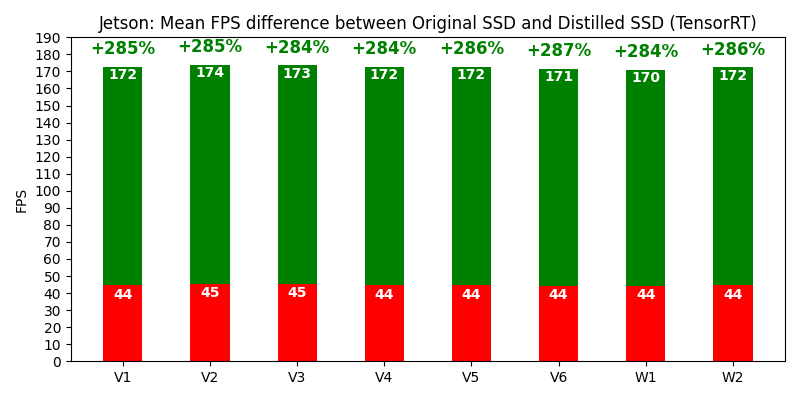
\includegraphics[width = \linewidth]{Mean Difference FPS Jetson TensorRT.png}
    \centering
    \caption{Benchmark media differenza FPS tra i modelli SSD e DSSD su architettura Jetson Nano (TensorRT)}
    \label{bench-jet-tensorrt}
\end{figure}
Lo stesso comportamento si verifica sia quando viene utilizzata OpenCV con supporto CUDA (cuDNN) (Fig. \ref{bench-jet-cv2-cudnn}) e sia quando OpenCV effettua una semplice inferenza su CPU (Fig. \ref{bench-jet-cv2-CPU}).
\begin{figure}
    \centering
    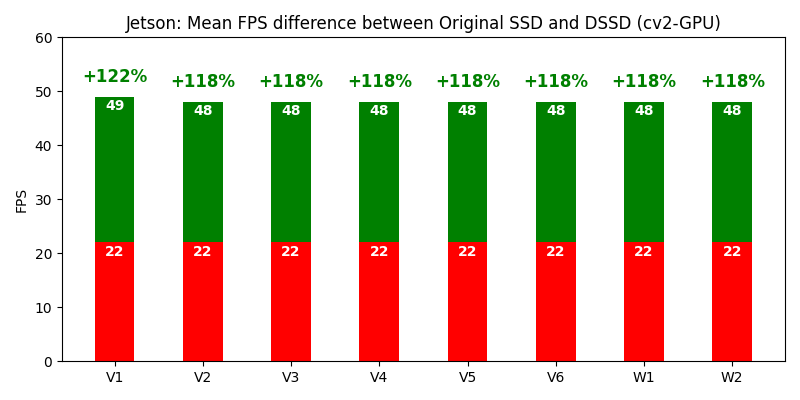
\includegraphics[width = \linewidth]{Difference FPS Jetson cv2 Cuda.png}
    \centering
    \caption{Benchmark media differenza FPS tra i modelli SSD e DSSD su architettura Jetson Nano (OpenCV - cuDNN)}
    \label{bench-jet-cv2-cudnn}
\end{figure}
\begin{figure}
    \centering
    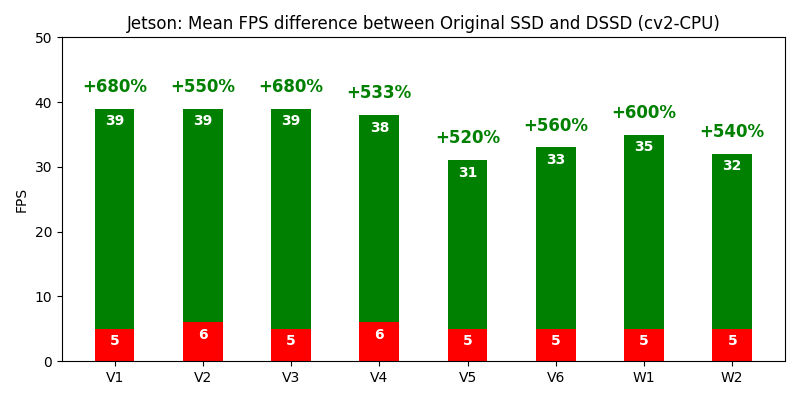
\includegraphics[width = \linewidth]{Difference FPS Jetson cv2 CPU.png}
    \centering
    \caption{Benchmark media differenza FPS tra i modelli SSD e DSSD su architettura Jetson Nano (OpenCV - CPU)}
    \label{bench-jet-cv2-CPU}
\end{figure}

\subsubsection{Benchmarks DSSD sul Computer}
Cambiando tipologia di architettura, quando ci si sposta sul computer bisogna ricordarsi che non è possibile utilizzare alcun acceleratore grafico in quanto non vi è un supporto CUDA. Stando a tale limitazione, i test vengono effettuati con l'utilizzo di OpenCV che esegue l'inferenza sulla sola CPU. I risultati ottenuti sono mostrati nella Figura \ref{bench-pc-cv2-CPU}.
\begin{figure}
    \centering
    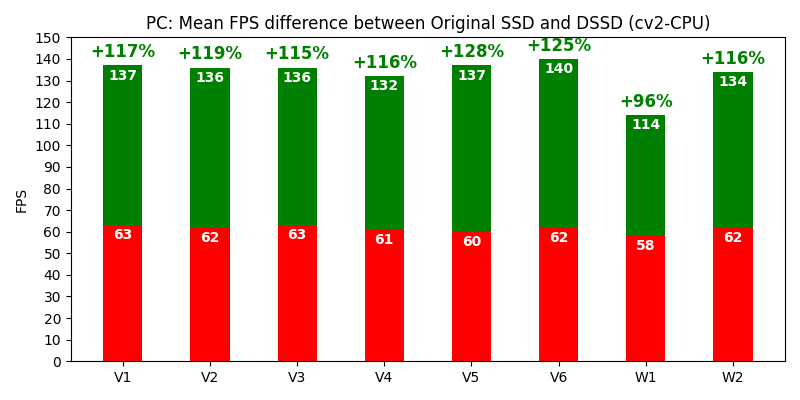
\includegraphics[width = \linewidth]{Mean Difference FPS pc only CPU.png}
    \centering
    \caption{Benchmark media differenza FPS tra i modelli SSD e DSSD su architettura Apple Macbook Pro (OpenCV - CPU)}
    \label{bench-pc-cv2-CPU}
\end{figure}

\subsubsection{Benchmarks DSSD su Google Colaboratory}
Spostandoci all'ultima architettura, rispetto alle precedenti ha la possibilità di utilizzare solamente OpenCV per l'inferenza dei modelli. In questo caso, vengono effettuate due tipologie di benchmarks, entrambi utilizzando OpenCV. 
Le performance ottenute dall'inferenza eseguita sulla GPU, e quindi utilizzando il supporto cuDNN di OpenCV, sono riportate nella Figura \ref{bench-colab-cv2-cudnn}.
\begin{figure}
    \centering
    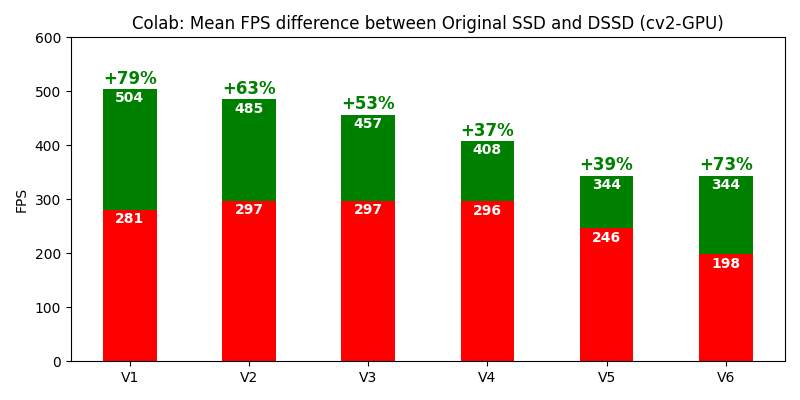
\includegraphics[width = \linewidth]{Mean Difference FPS Colab only GPU.png}
    \centering
    \caption{Benchmark media differenza FPS tra i modelli SSD e DSSD su architettura Google Colaboratory (OpenCV - cuDNN)}
    \label{bench-colab-cv2-cudnn}
\end{figure}
Infine, l'ultimo test è stato eseguito sulla sola CPU di Google Colab, sempre utilizzando OpenCV senza alcun acceleratore, ottenendo delle performance visibili in Figura \ref{bench-colab-cv2-cpu}.
\begin{figure}
    \centering
    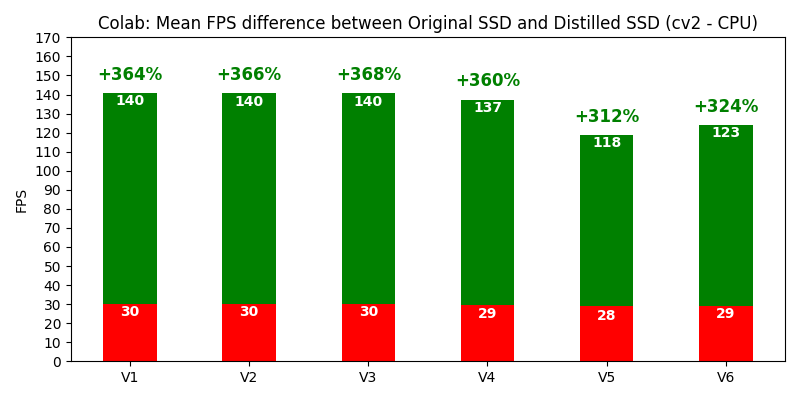
\includegraphics[width = \linewidth]{Mean Difference FPS Colab only CPU.png}
    \centering
    \caption{Benchmark media differenza FPS tra i modelli SSD e DSSD su architettura Google Colaboratory (OpenCV - CPU)}
    \label{bench-colab-cv2-cpu}
\end{figure}

\section{Esempi Object Detection modello DSSD}
Fino a questo punto sono stati mostrati tutti i benefici derivanti dal nuovo modello proposto DSSD. Tutti i dati sono incoraggianti per l'adozione di tale rete su varie architetture embedded e non. Dal punto di vista pratico però, non sono state ancora dimostrare le effettive funzionalità offerte dal modello. Nella seguente sezione, che termina il capitolo corrente, vengono mostrati alcuni esempi, inerenti l'attività di object detection, prodotti dal modello DSSD. Per capire meglio le differenze in tale attività, rispetto al modello insegnante SSD, vengono confrontati i risultati ottenuti sulle stesse immagini in cui saranno visibili i riquadri di delimitazione di ogni oggetto (bounding-boxes) e i corrispettivi valori percentuali attribuiti ad ogni classe predetta. 
Le immagini utilizzate provengono dal dataset Open Images.
Guardando attentamente i punteggi generati, il modello DSSD, essendo ricavato dalla tecnica di Knowledge Distillation\index{Knowledge Distillation}, non avrà mai la stessa accuratezza dell'insegnante. Questo fattore dipende soprattutto dall'applicazione della temperatura influenzante la generazione delle soft-labels. 
Tuttavia, il modello DSSD produce risultati che non si discostano tanto da quelli del modello insegnante. Tali risultati dimostrano come la tecnica di Knowledge Distillation\index{Knowledge Distillation} riesca quasi a preservare l'accuratezza proveniente dal modello insegnante. 
\begin{figure}[ht] 
    \begin{subfigure}[b]{0.5\linewidth}
      \centering
      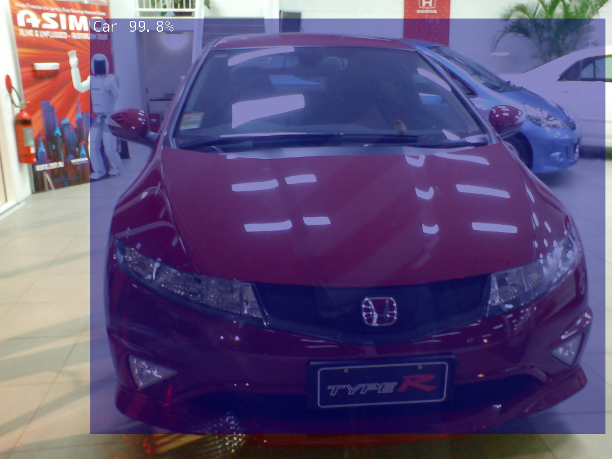
\includegraphics[width=0.9\linewidth]{Compare 1 T.png} 
      \label{fig7:a} 
    \end{subfigure}%% 
    \begin{subfigure}[b]{0.5\linewidth}
      \centering
      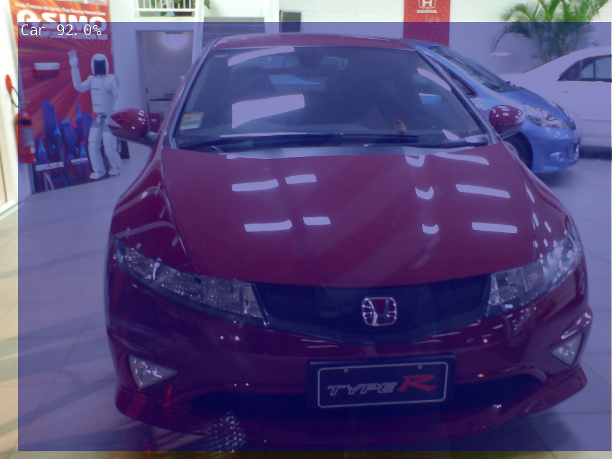
\includegraphics[width=0.9\linewidth]{Compare 1 S.png} 
      \label{fig7:b} 
    \end{subfigure} 
    \begin{subfigure}[b]{0.5\linewidth}
      \centering
      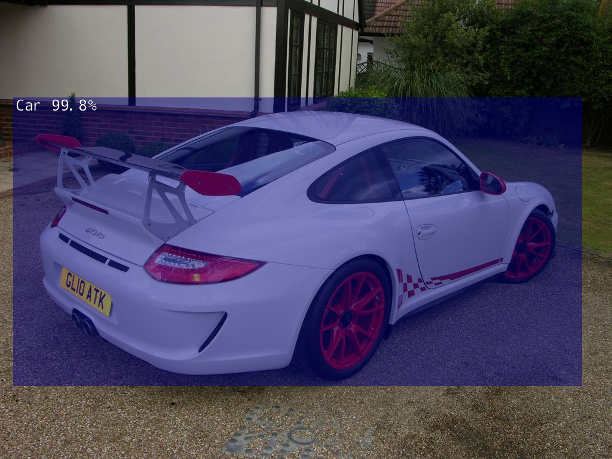
\includegraphics[width=0.9\linewidth]{Compare 2 T.png} 
      \label{fig7:c} 
    \end{subfigure}%%
    \begin{subfigure}[b]{0.5\linewidth}
      \centering
      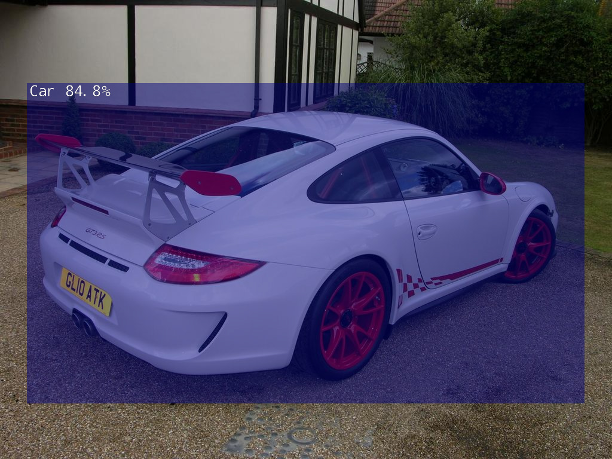
\includegraphics[width=0.9\linewidth]{Compare 2 S.png} 
      \label{fig7:d} 
    \end{subfigure}
    \begin{subfigure}[b]{0.5\linewidth}
        \centering
        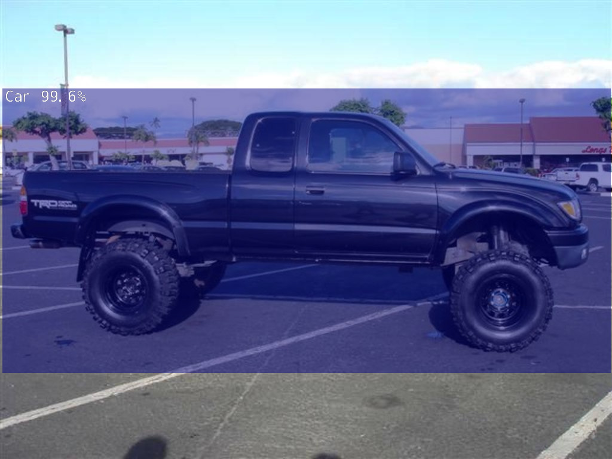
\includegraphics[width=0.9\linewidth]{Compare 3 T.png} 
        \caption{Output SSD Insegnante} 
        \label{fig7:d} 
    \end{subfigure}%%
    \begin{subfigure}[b]{0.5\linewidth}
        \centering
        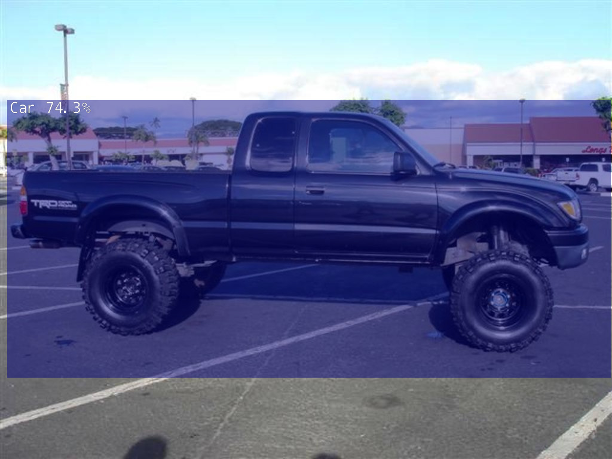
\includegraphics[width=0.9\linewidth]{Compare 3 S.png} 
        \caption{Output DSSD} 
        \label{fig7:d} 
    \end{subfigure}
    \caption{Comparazione visiva output SSD insegnante (a) e output DSSD (b).}
    \label{fig7} 
\end{figure}

